%% Based on a TeXnicCenter-Template by Gyorgy SZEIDL.
%%%%%%%%%%%%%%%%%%%%%%%%%%%%%%%%%%%%%%%%%%%%%%%%%%%%%%%%%%%%%

%----------------------------------------------------------
%

%
%----------------------------------------------------------
% This is a sample document for the LaTeX Slides Class
% Class options
%       --  Body text point size (normalsize) is 27 (default)
%           and can not be adjusted to any other value.
%       --  Paper size:  letterpaper (8.5x11 inch, default)
%                        a4paper, a5paper, b5paper,
%                        legalpaper, executivepaper
%       --  Orientation (portrait is the default):
%                        landscape
%       --  Quality:     final(default), draft
%       --  Title page:  titlepage, notitlepage
%       --  Columns:     onecolumn (default), [twocolumn is not avalible]
%       --  Equation numbering (equation numbers on the right is the default)
%                        leqno (equation numbers on the left)
%       --  Displayed equations (centered is the default)
%                    fleqn (flush left)
%
%  \documentclass[a4paper,fleqn]{slides}
%
%  The slides are separated from each other by the slide
%  environment, see below:
%


\PassOptionsToPackage{table}{xcolor}
\documentclass[xcolor=dvipsnames]{beamer}
\usepackage[latin1]{inputenc}
\usepackage[T1]{fontenc}
\usepackage[ngerman]{babel}
\usepackage{amsmath}
\usepackage{amssymb,amsfonts,textcomp}
%\usepackage{array}
%\usepackage{hhline}
%\usepackage{lmodern}
%%\usepackage{epsfig}
\usepackage{graphics}
%\usepackage{exscale} %Skalierung der Mathesymbole
%\usepackage{ifthen}
%\usepackage{epic,eepic}
\usepackage{color}
%\usepackage{hyperref}
\usepackage[absolute,overlay]{textpos}
%\usepackage{booktabs}
%\usepackage{url}
\usepackage{tikz}
\usetikzlibrary{arrows,shapes,positioning}
\usetikzlibrary{calc}
\usetikzlibrary{mindmap,shadows,trees}

\usetheme{PaloAlto}
\useinnertheme{rounded}
%\definecolor{tuc}{cmyk}
%\definecolor{tuc}{RGB}{0,90,70}
%\definecolor{tuc}{RGB}{23,118,101}%{40,128,255} %
\definecolor{tuc}{RGB}{255,255,9}
\usecolortheme[named=tuc]{structure}

%%% --------------------------------------------------------------
\setbeamercolor{title}{fg=black}
\setbeamercolor{title in sidebar}{fg=black}
\setbeamercolor{author in sidebar}{fg=black}
\setbeamercolor{subsection in sidebar}{fg=black}
\setbeamercolor{section in sidebar}{fg=black}
\setbeamercolor{frametitle}{fg=black}

\logo{
\includegraphics[width=1.5cm]{chch.png}}



\begin{document}
\title{Es gibt viel zu tun -- hau'n wir ab.}
\author{Stefan Helmert}
\date{03.05.2014}
%\maketitle
% ----------------------------------------------------------------


\frame{\titlepage 
	\begin{textblock}{5}(11,10)
		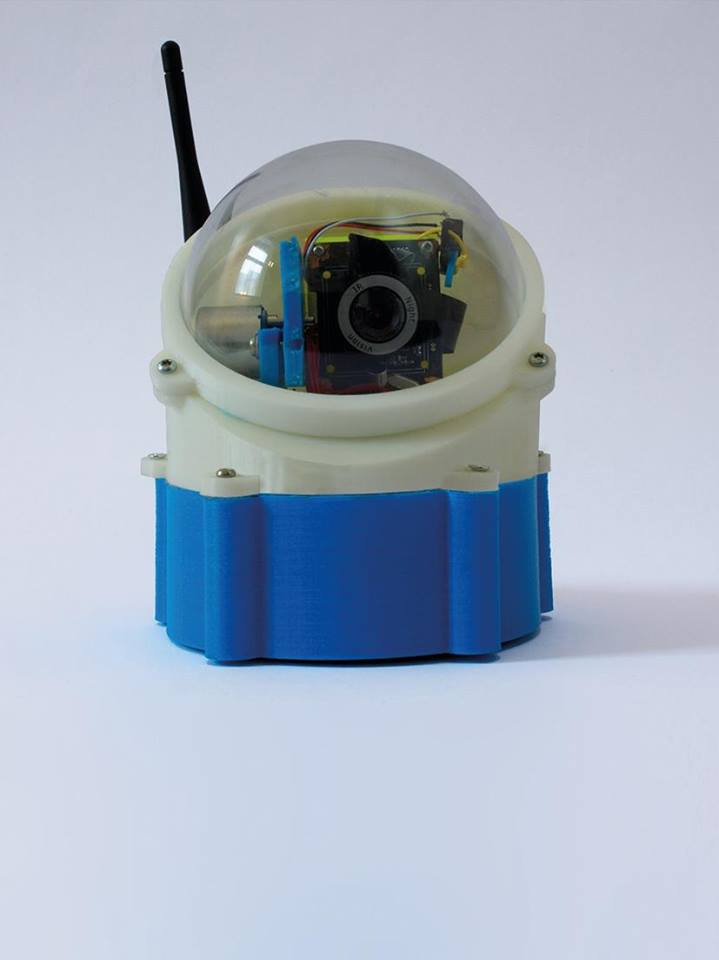
\includegraphics[width=3cm]{Kamera.jpg}	
	\end{textblock}
}


\section{Zutaten}
\frame{\frametitle{Viele Sachen...}
	\includegraphics[height=7.5cm]{Pcs.jpg}	
}
\frame{\frametitle{Netzwerk}
	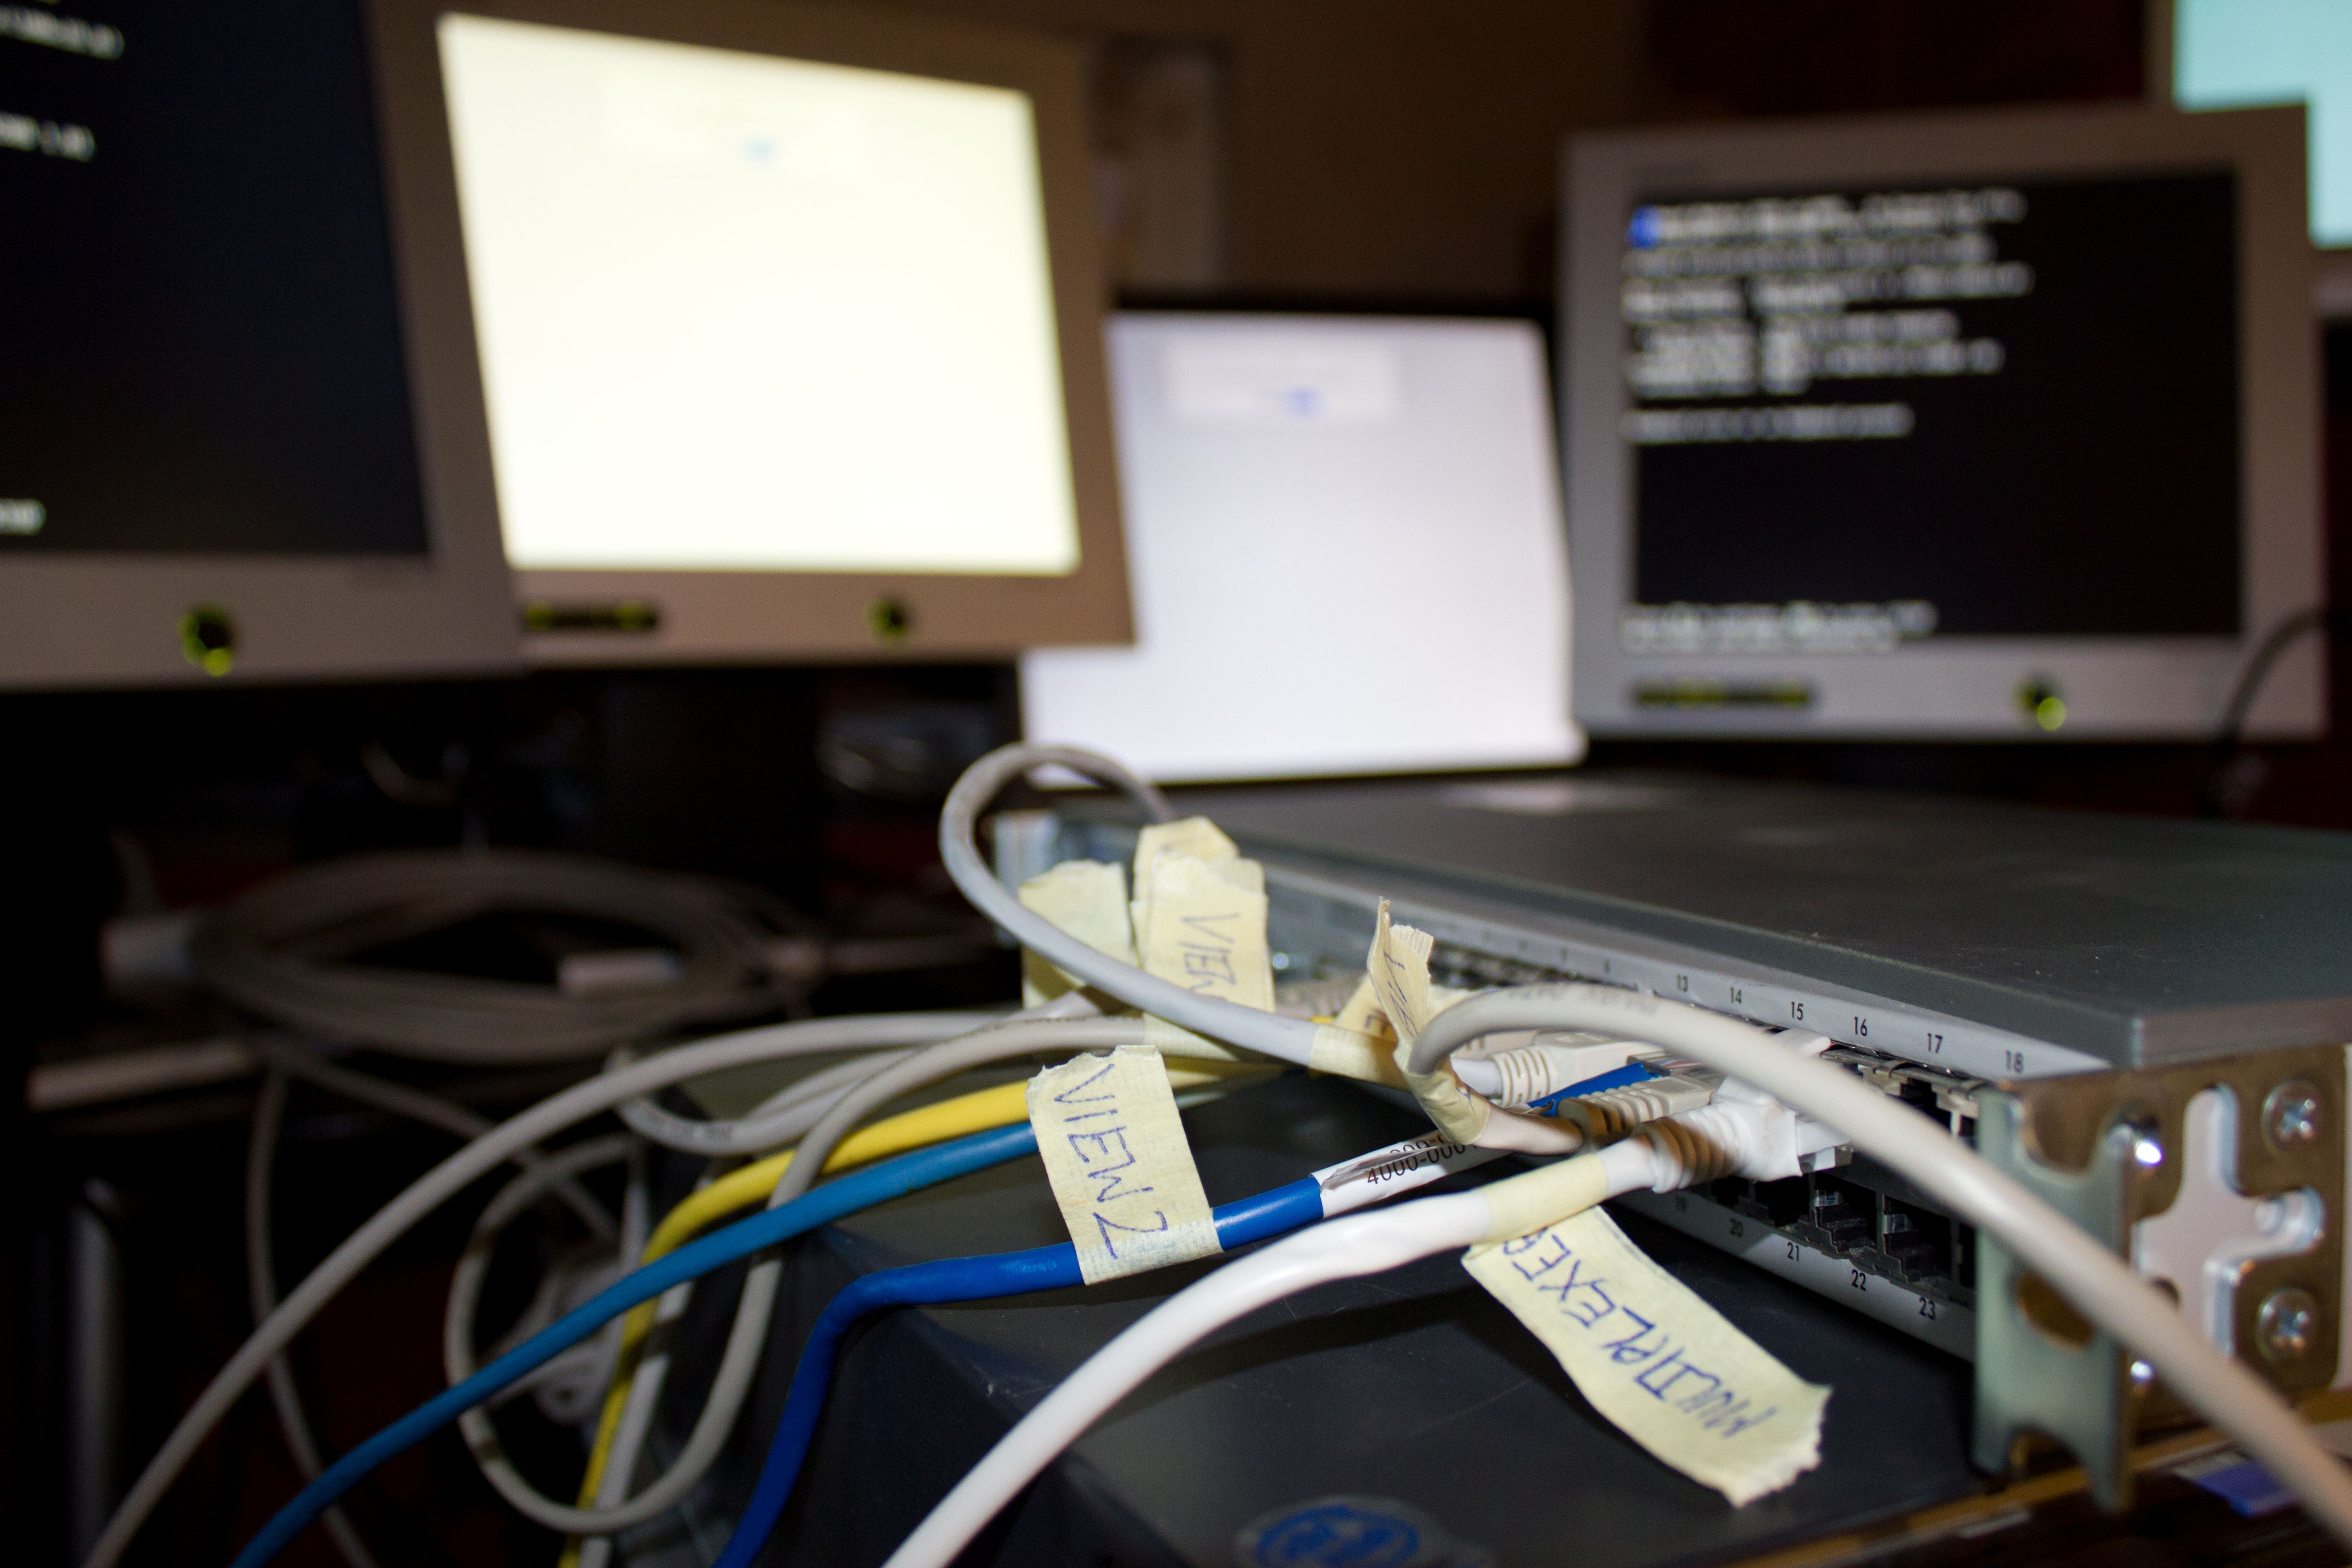
\includegraphics[width=10cm]{Netzwerk.jpg}	
}
\frame{\frametitle{Drahtlos}
	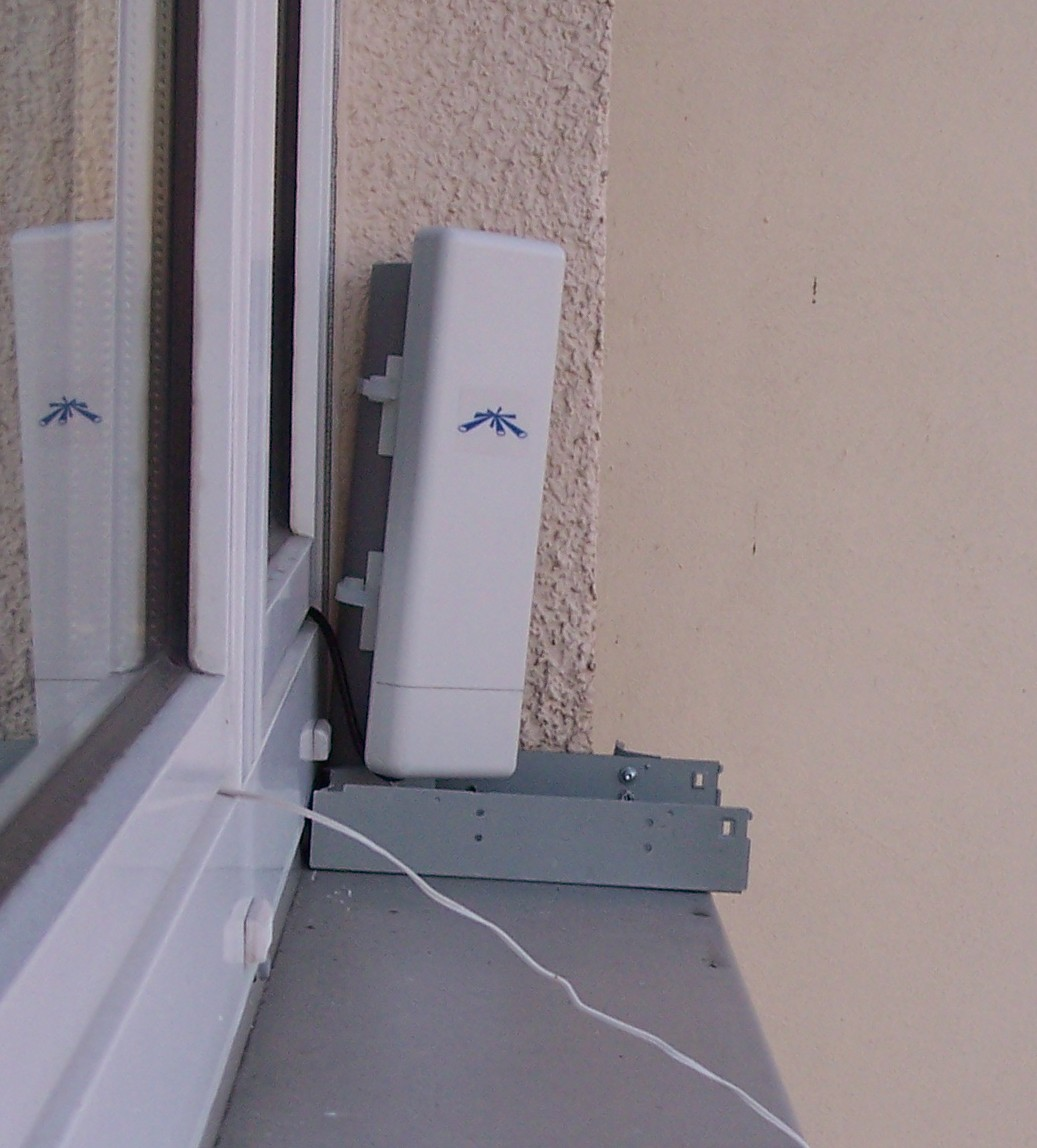
\includegraphics[height=7.5cm]{NS5.jpg}	
}
\frame{\frametitle{Kamera}
	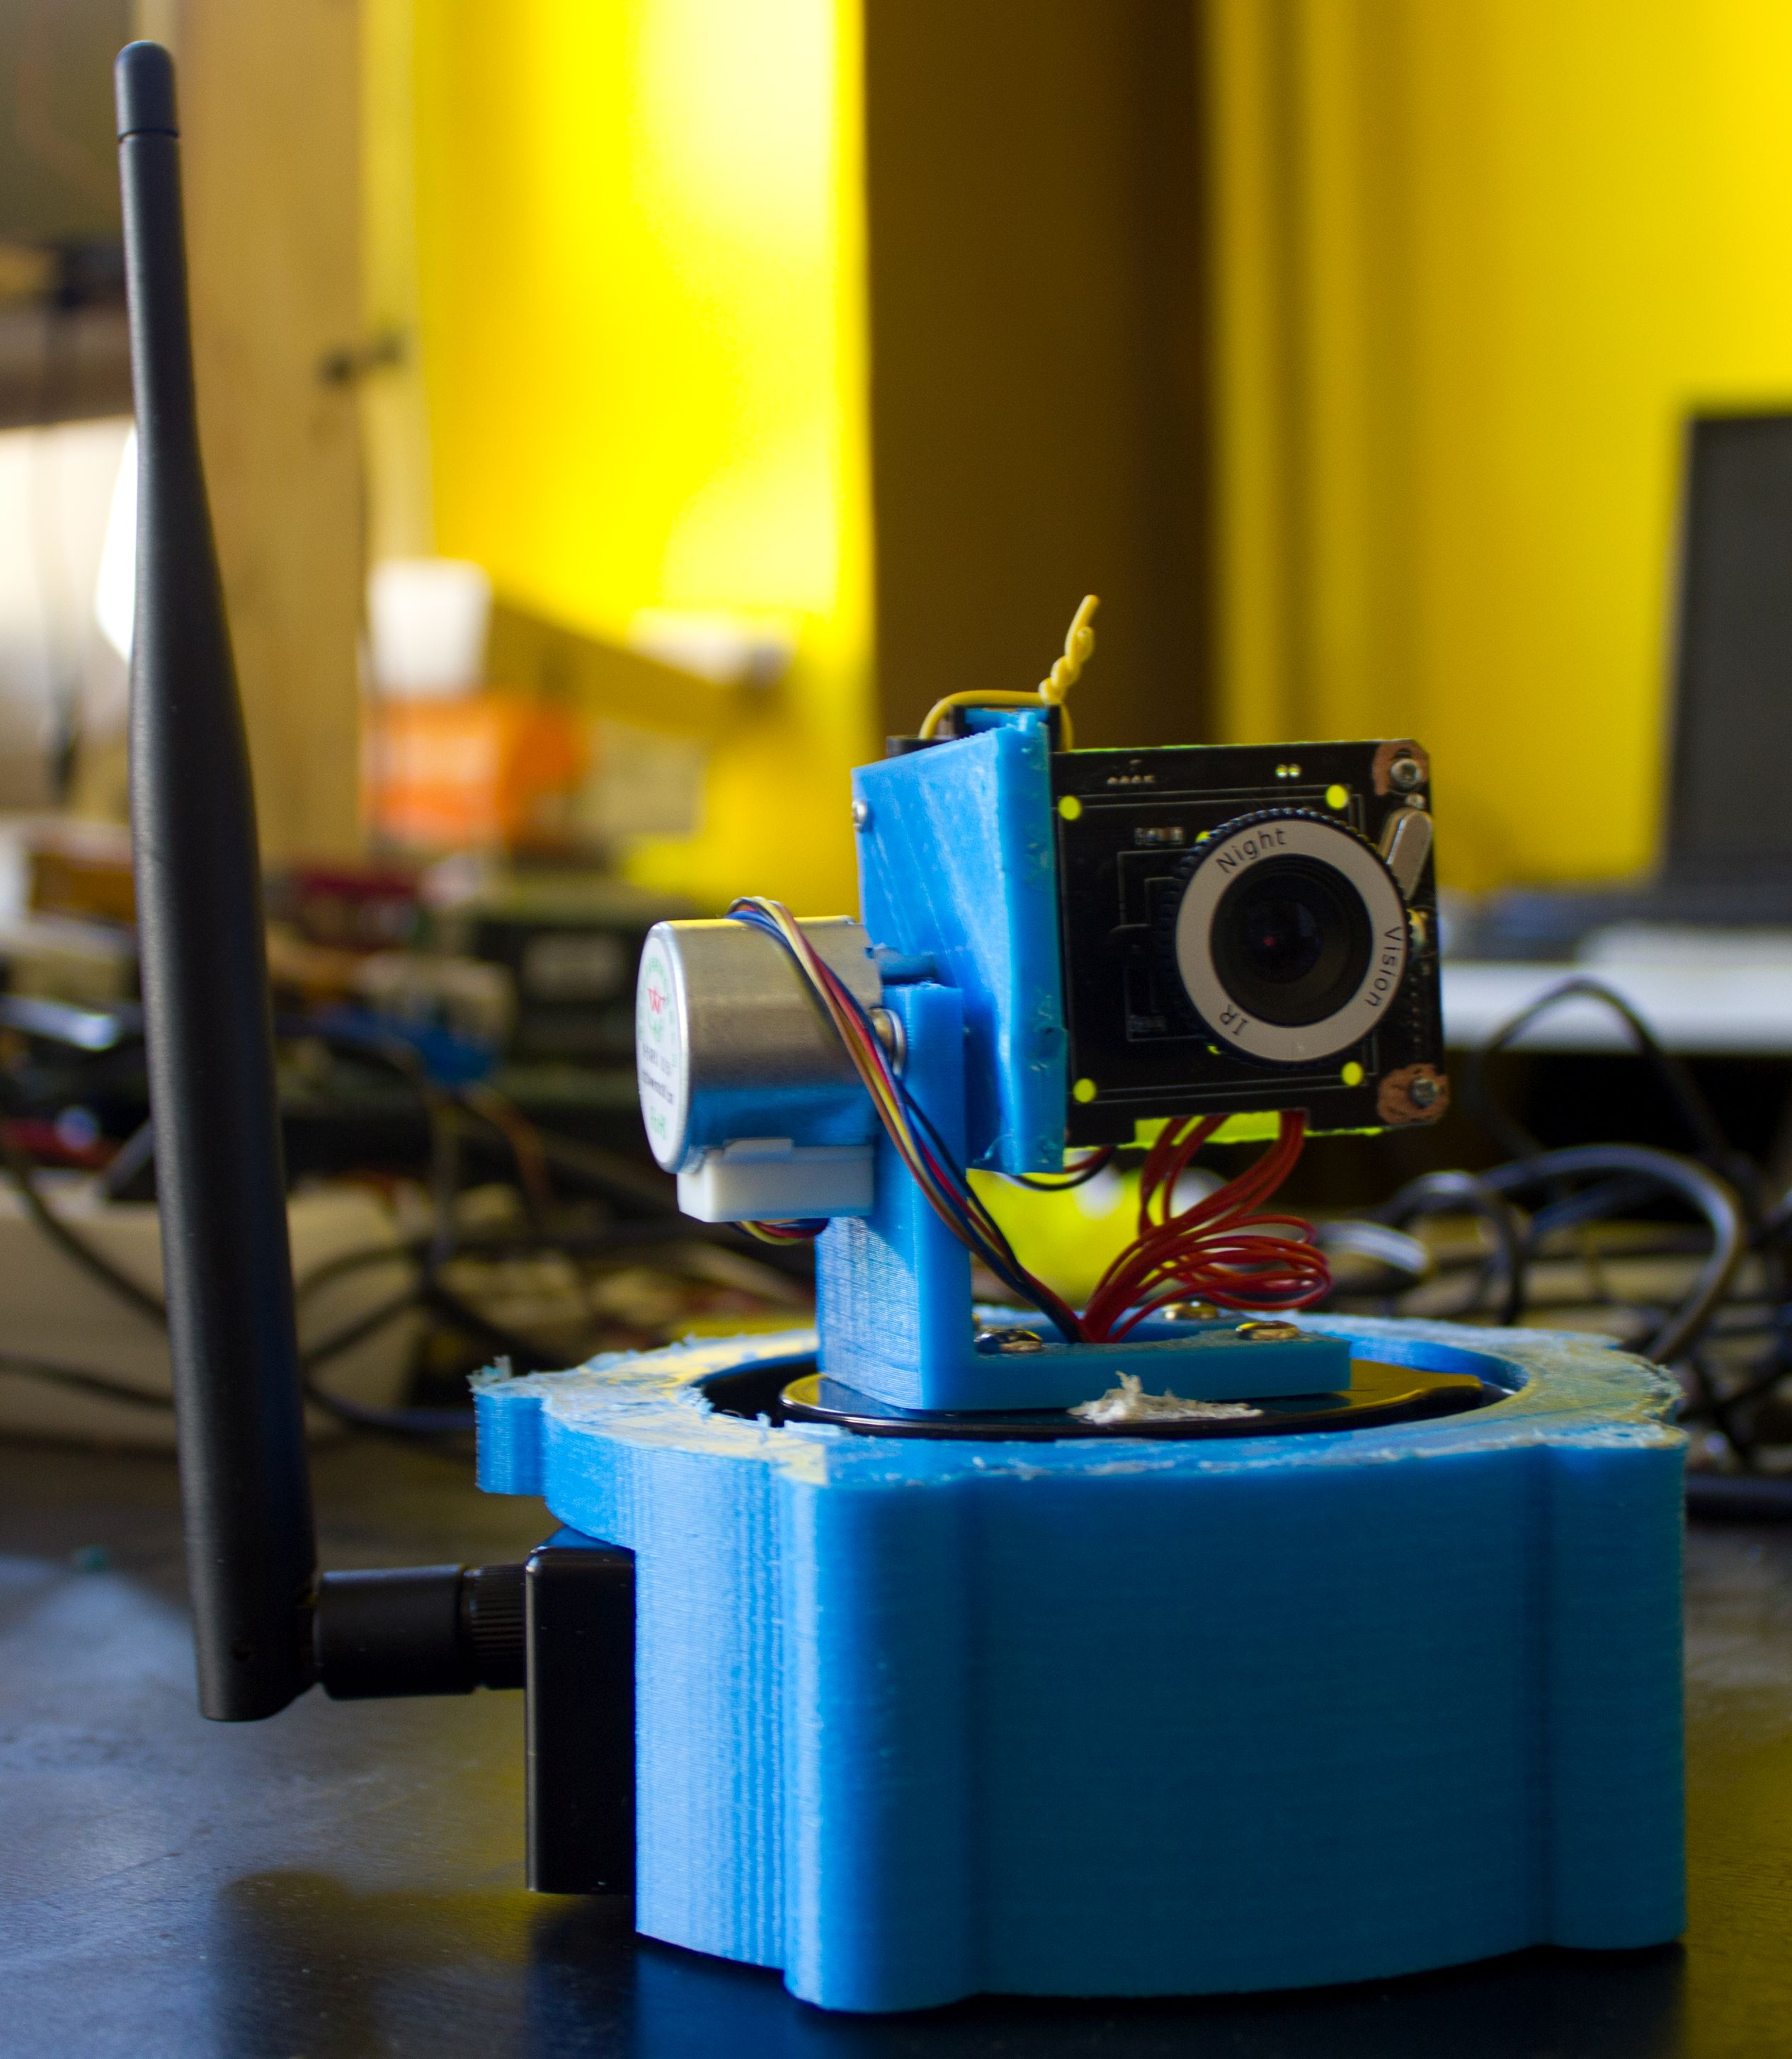
\includegraphics[height=7.5cm]{Cam.jpg}	
}
\frame{\frametitle{Software}
	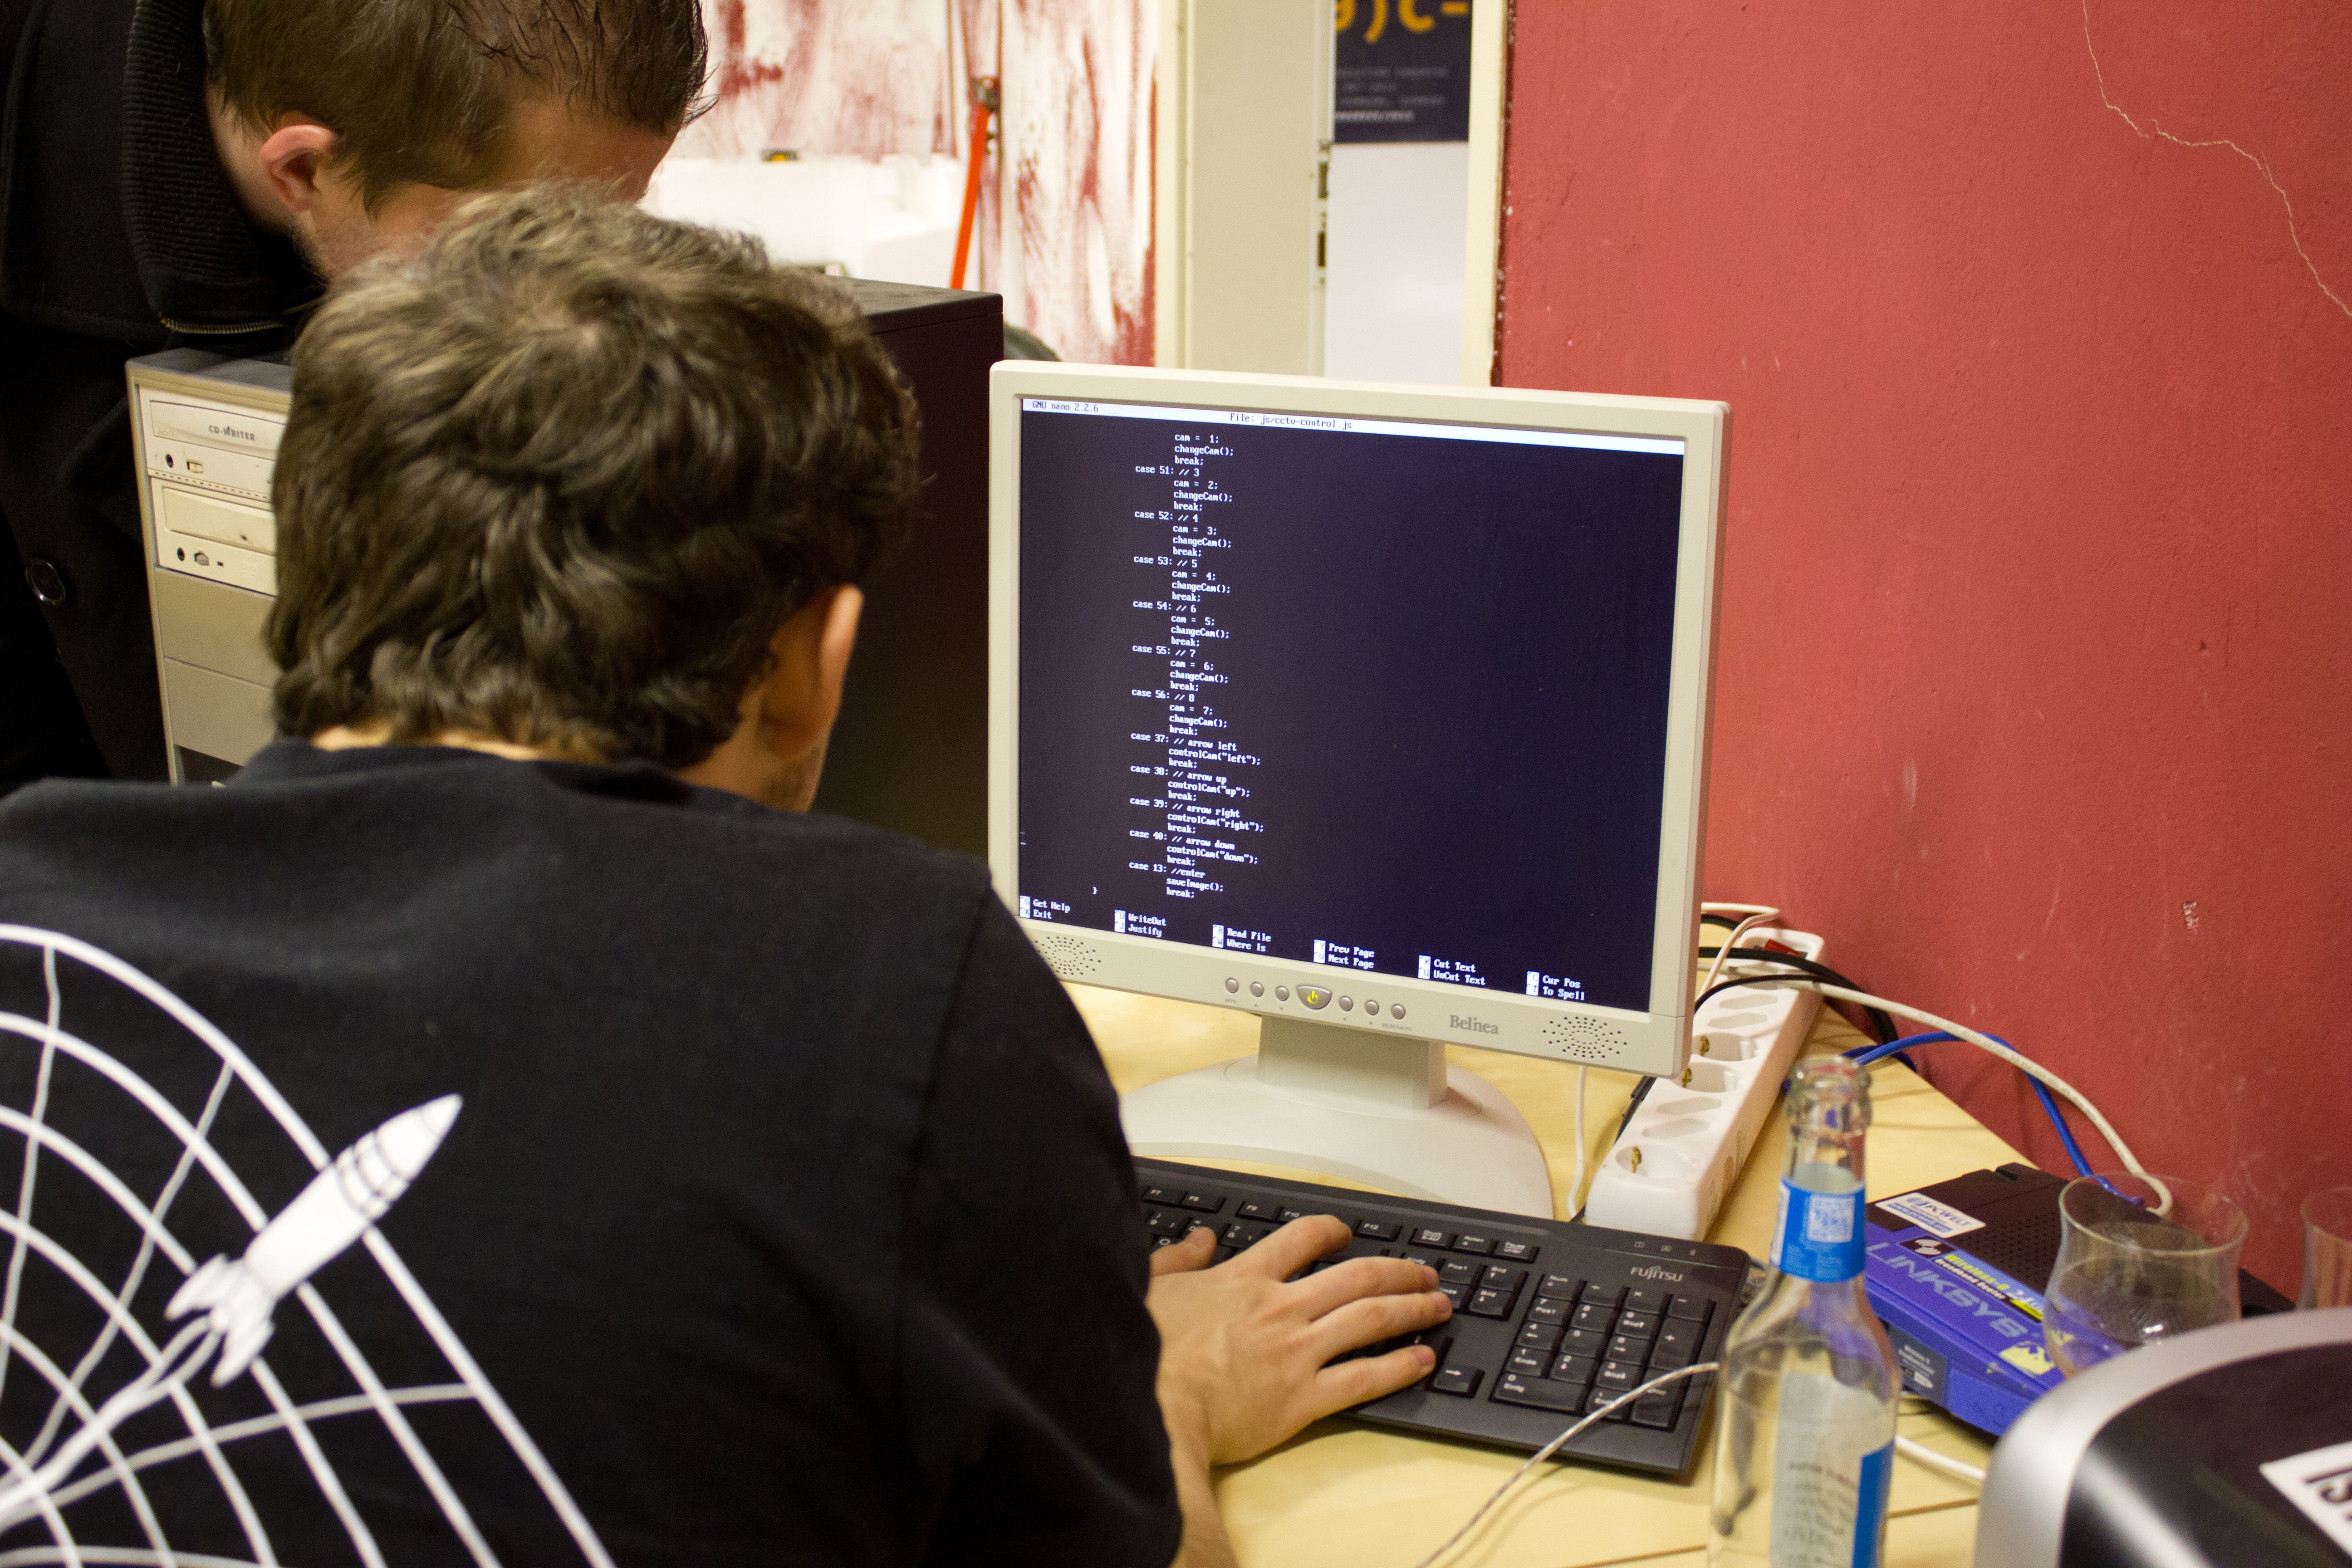
\includegraphics[width=10cm]{Software.jpg}	
}
\frame{\frametitle{Panzer}
	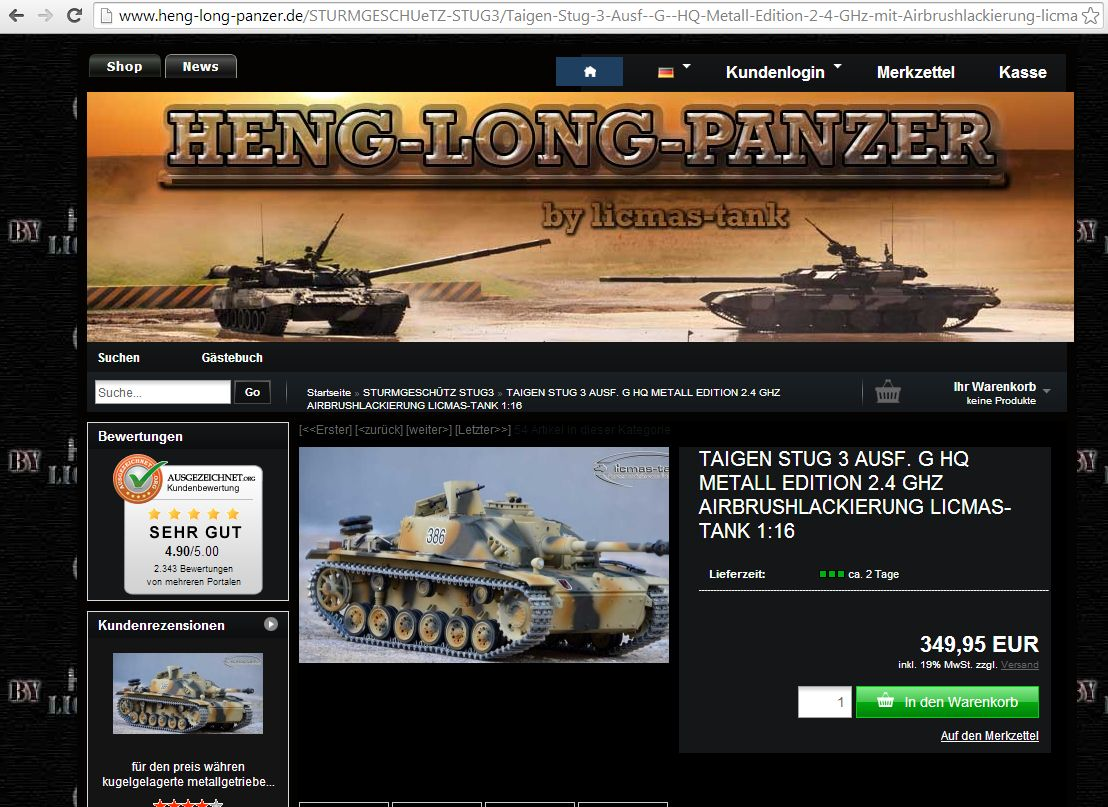
\includegraphics[width=10cm]{Panzer.jpg}	
}
\frame{\frametitle{Roboter}
	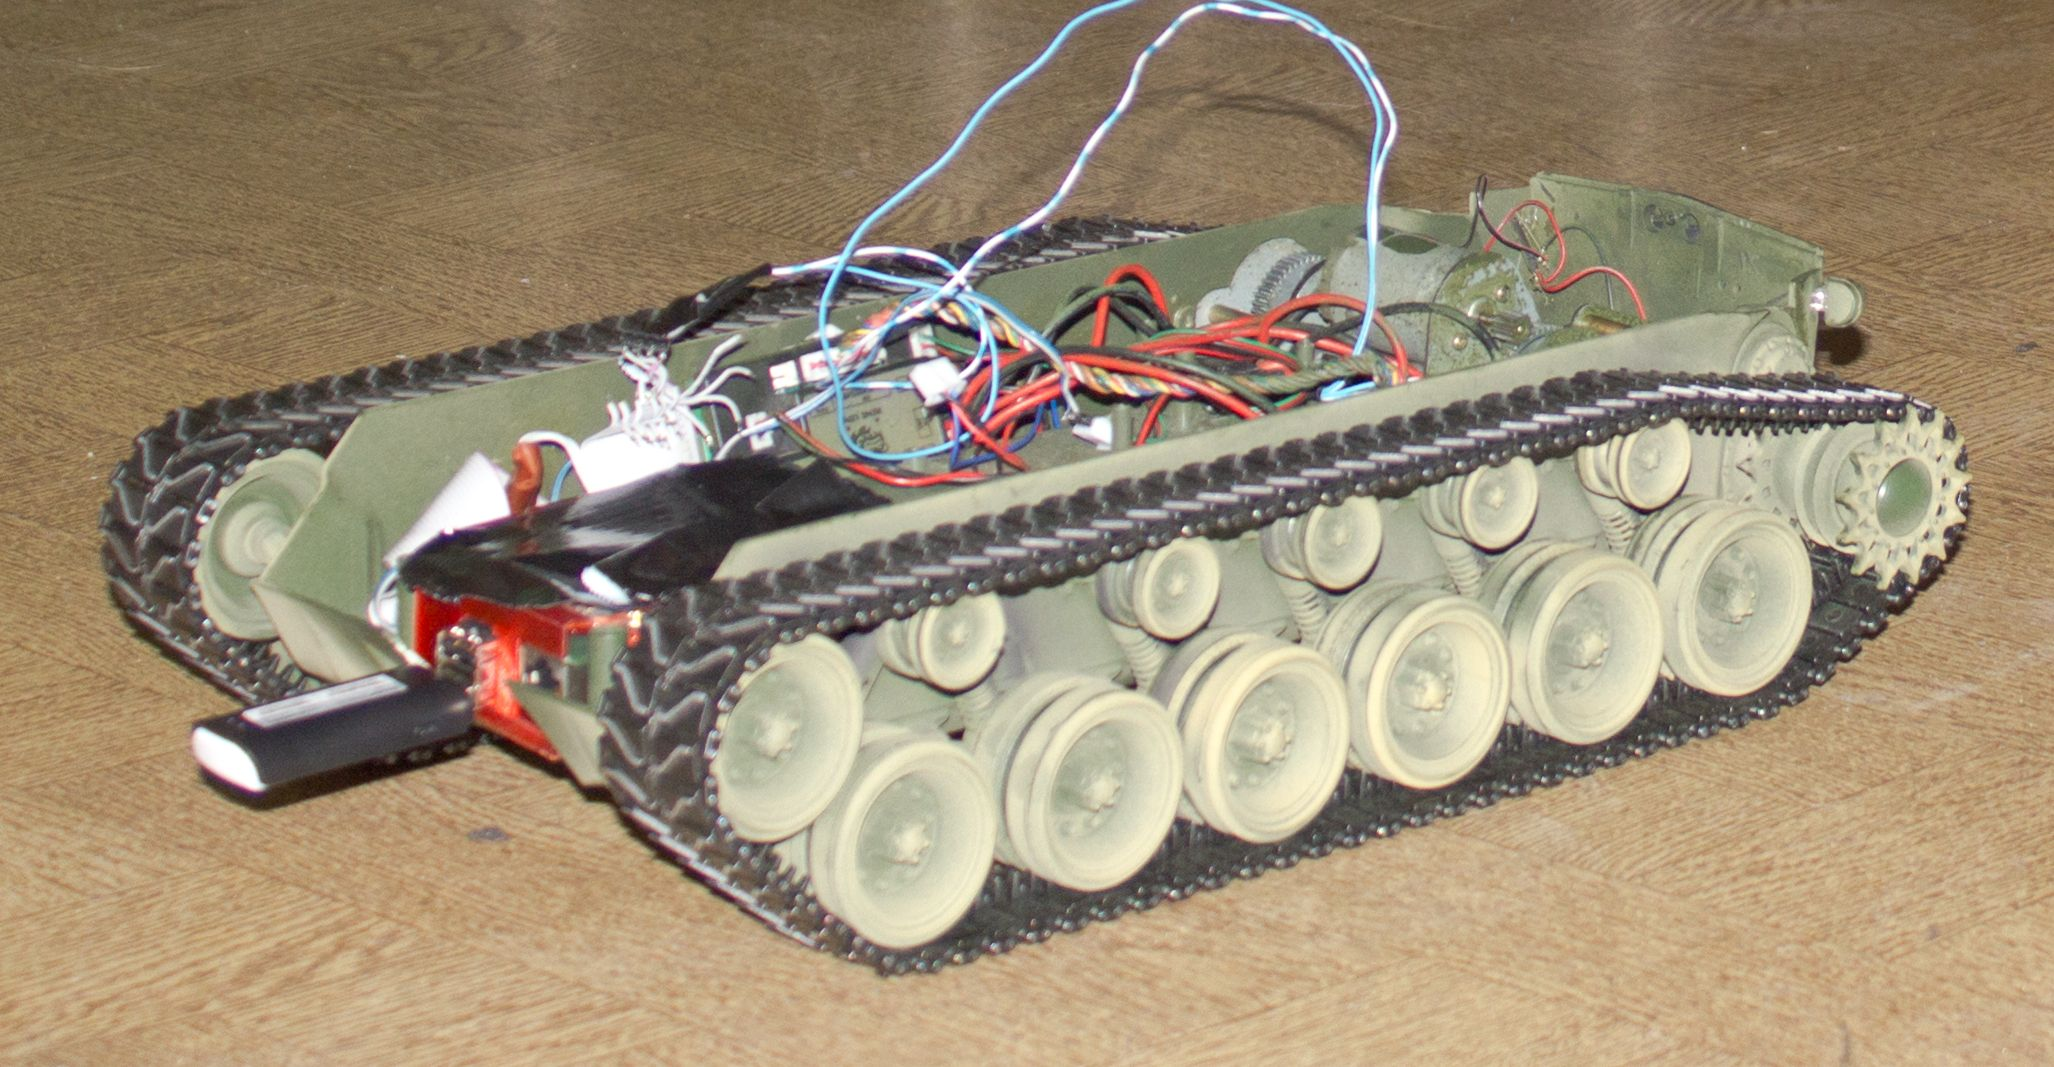
\includegraphics[width=10cm]{Robo.jpg}	
}
\frame{\frametitle{Elektronik}
	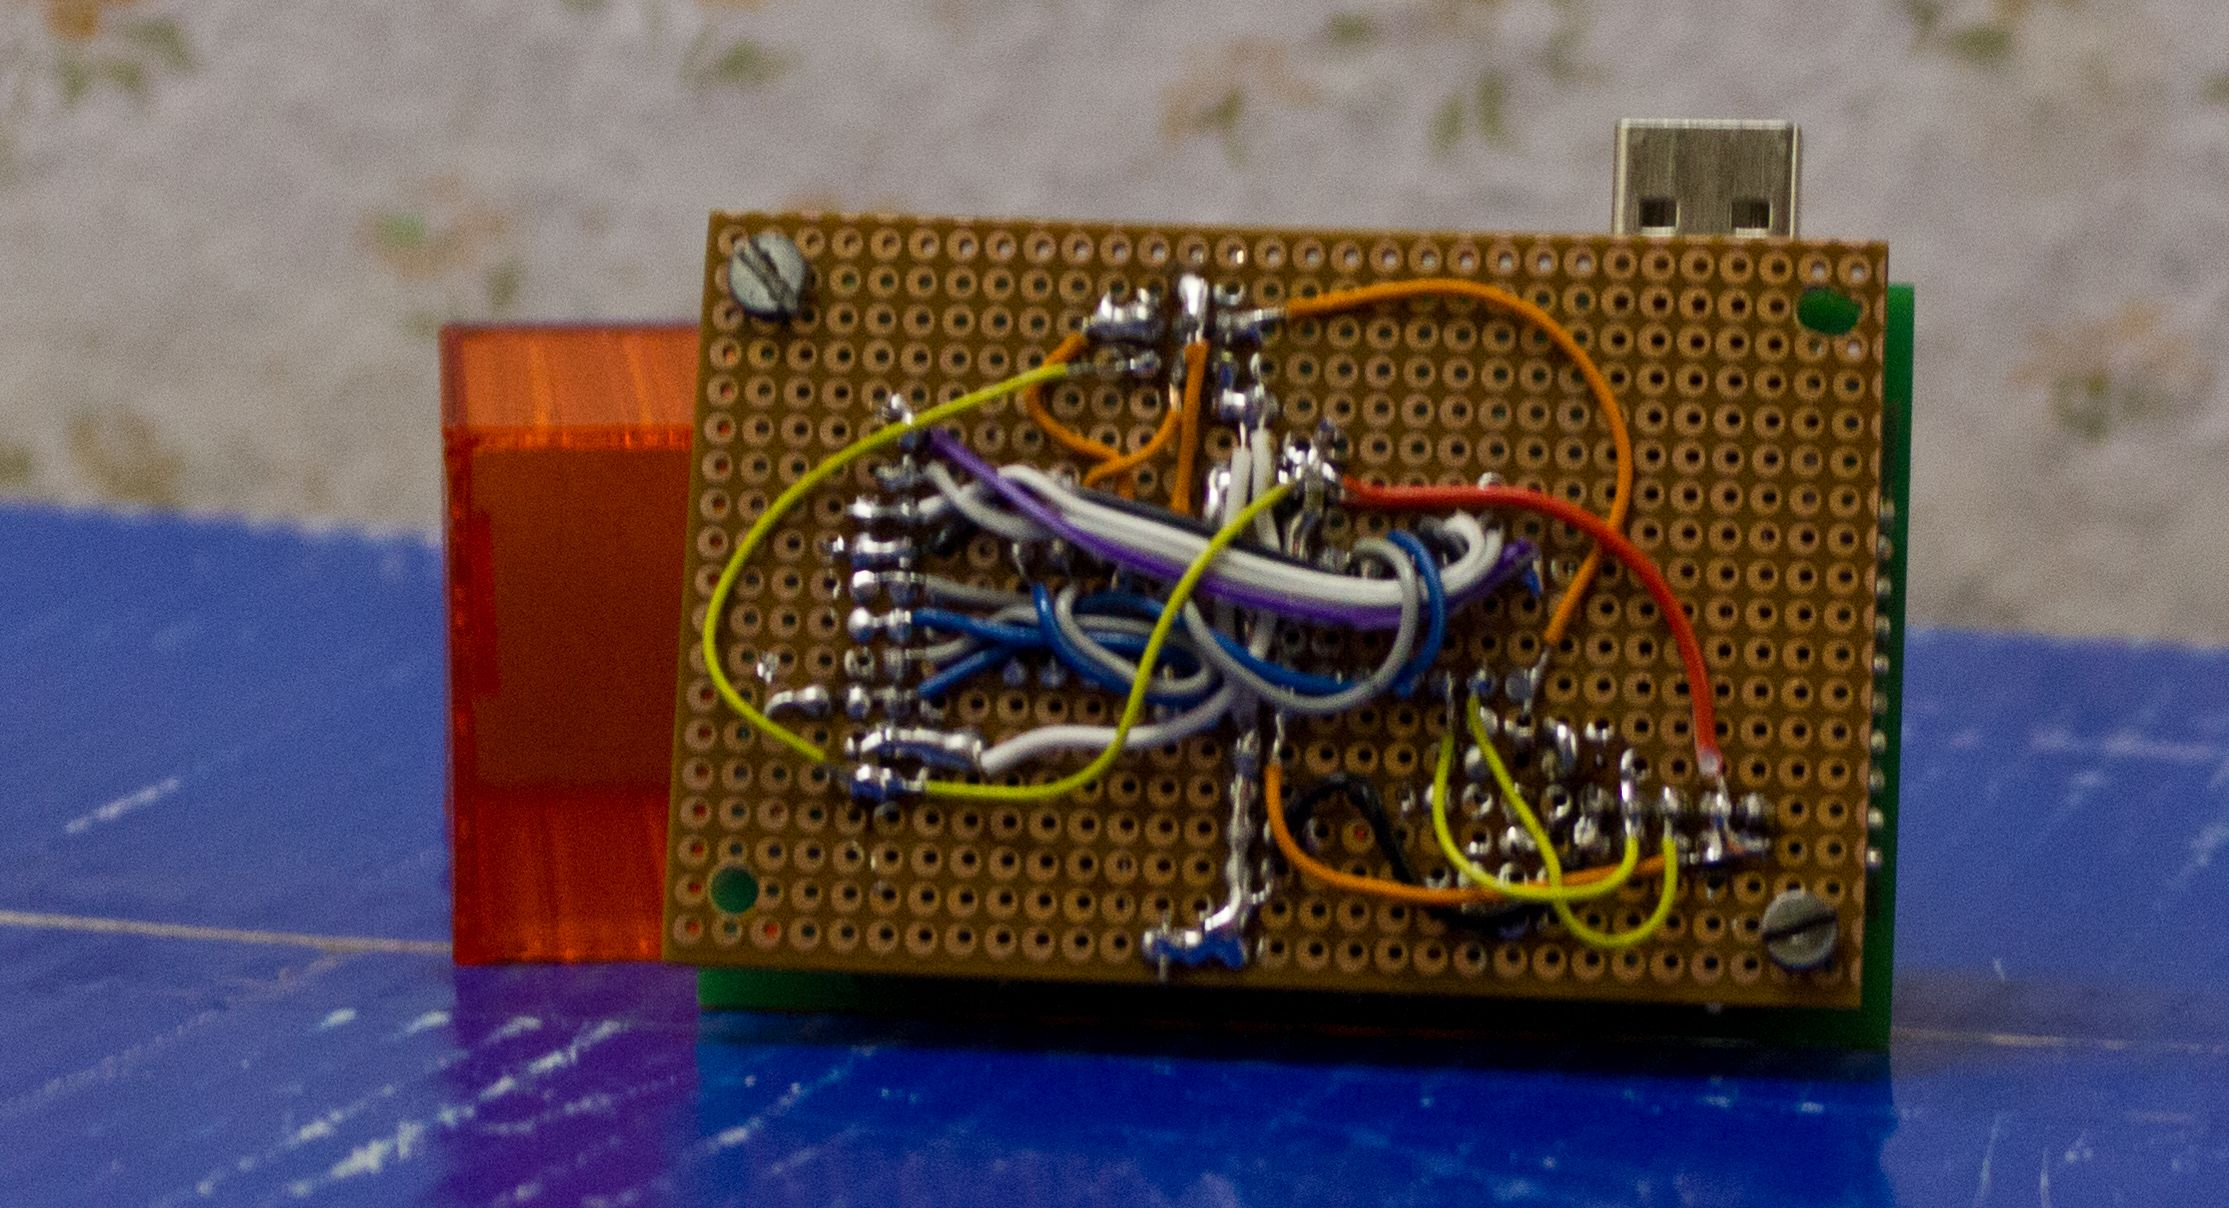
\includegraphics[width=10cm]{Elektronik.jpg}	
}
\frame
{
\frametitle{Material}
	\begin{itemize}
		\item Henglong-Panzer
		\item Filament f�r 3d-Drucker
		\item Kapton-Tape (oder Koptan ;))
		\item L�tzinn
		\item Schauben
		\item Besenstiel
		\item PCs mit Zubeh�r
		\item Netzwerkkabel
		\item IP-Kameras
		\item Gaffa-Tape
		\item Kabel 
		\item RaspberryPi
	\end{itemize}
	\textbf{Wir brauchen viele Sachen!}

}
\section{Organisation}
\frame{\frametitle{Es gibt viel zu tun...}
\begin{tikzpicture}[shorten >=1pt,auto,node distance=3cm,thick,minimum height=1.0cm]
	\node[ellipse,draw]	(men)	{12 Menschen};
	\node[]	(net) [below of=men] {Netzwerk};
	\node[]	(robo) [right of=net] {Roboter};
	\node[]	(stat) [left of=net] {�berwachungsstation};
	\node[]	(mech) [below of=net] {Mechanik};
	\node[]	(elec) [right of=mech] {Elektronik};
	\node[]	(soft) [left of=mech] {Software};
	\path[every node/.style={font=\sffamily\small}]
			(men) edge (net)
			(men) edge (robo)
			(men) edge (stat)
			(robo) edge (soft)
			(robo) edge (mech)
			(robo) edge (elec)
			(stat) edge (soft)
			(stat) edge (mech)
			(stat) edge (elec)
			(net) edge (soft)
			(net) edge (mech)
			(net) edge (elec)
			;
		\path[dashed] (stat) edge (net) (net) edge (robo);
\end{tikzpicture}
}
\section{Werkzeug}
\frame
{
\frametitle{Werkzeug}
	\textbf{Hardware}
	\begin{itemize}
		\item 3d-Drucker
		\item L�tkolben
		\item Schraubendreher
		\item Zangen
		\item Bohrschleifer 
		\item Computer
	\end{itemize}
	\textbf{Software}
	\begin{itemize}
		\item Openscad
		\item Cura
		\item Octoprint
		\item Codeblocks, gcc
		\item Linux
		\item Node.js
	\end{itemize}
}
\frame{\frametitle{3D-Drucker}
	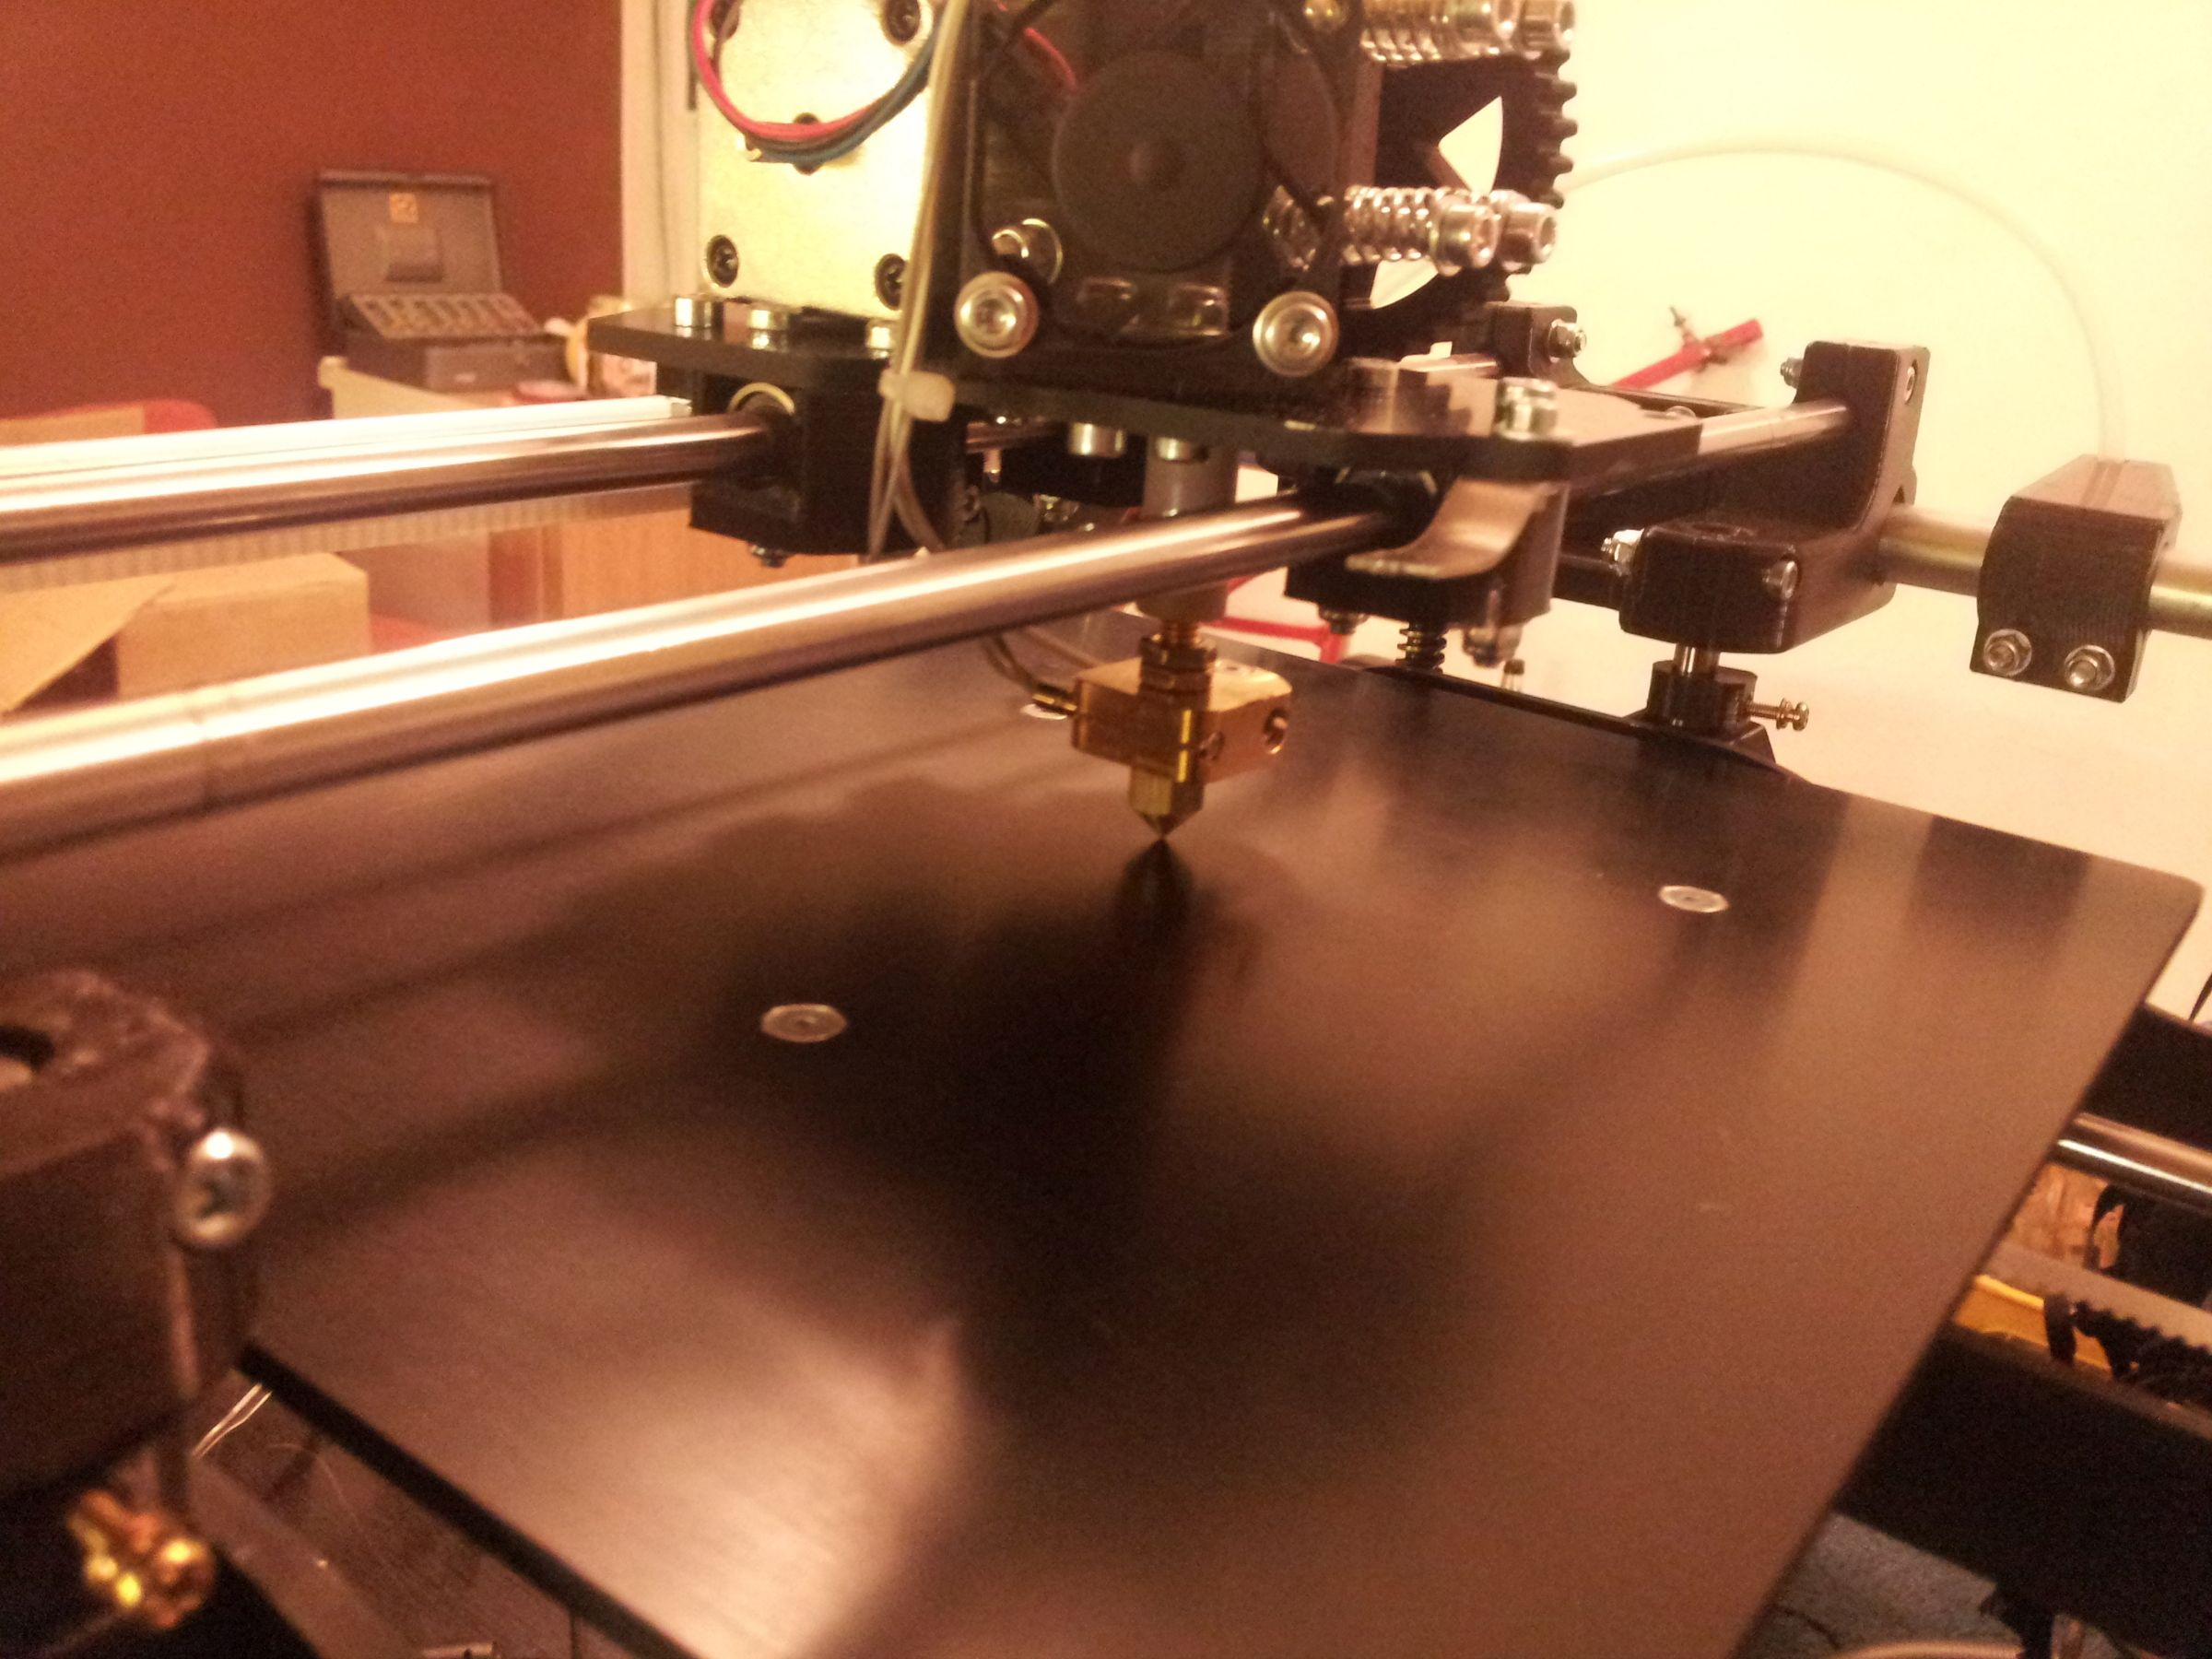
\includegraphics[width=10cm]{3D-Drucker.jpg}	
}
\frame{\frametitle{Roboter mit Kamera}
	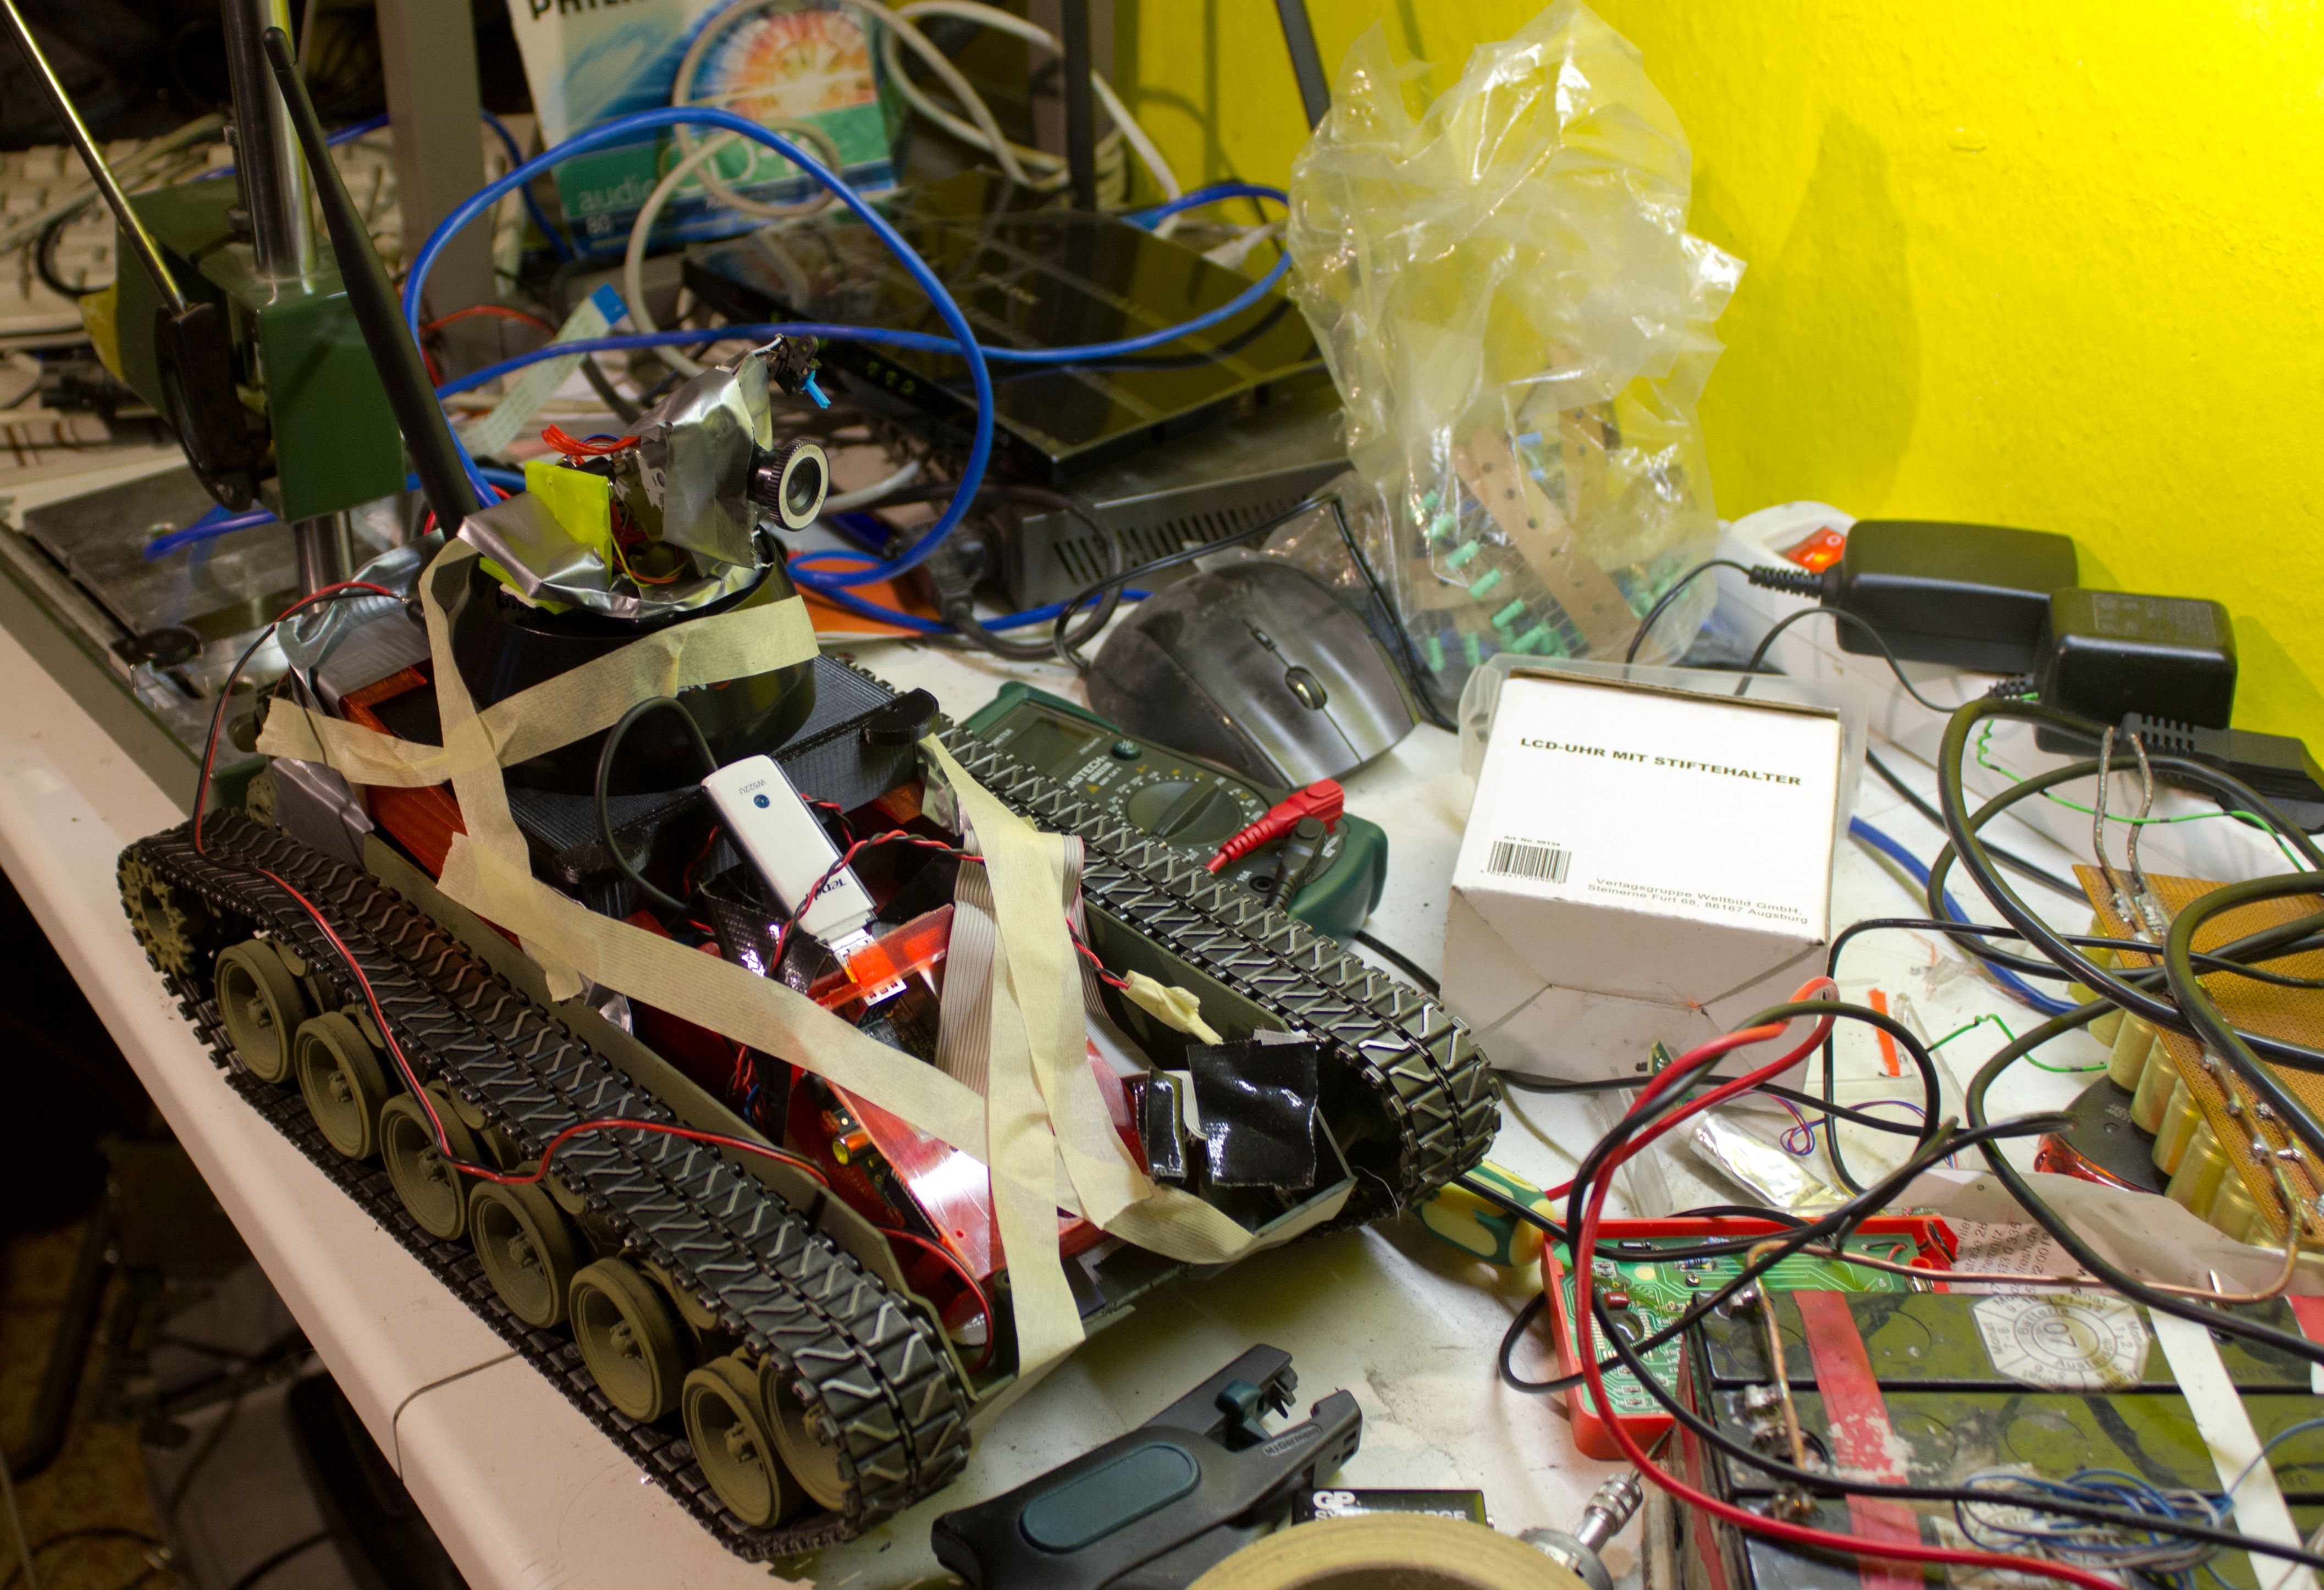
\includegraphics[width=10cm]{Robobesser.jpg}	
}
\frame{\frametitle{Besenstiel}
	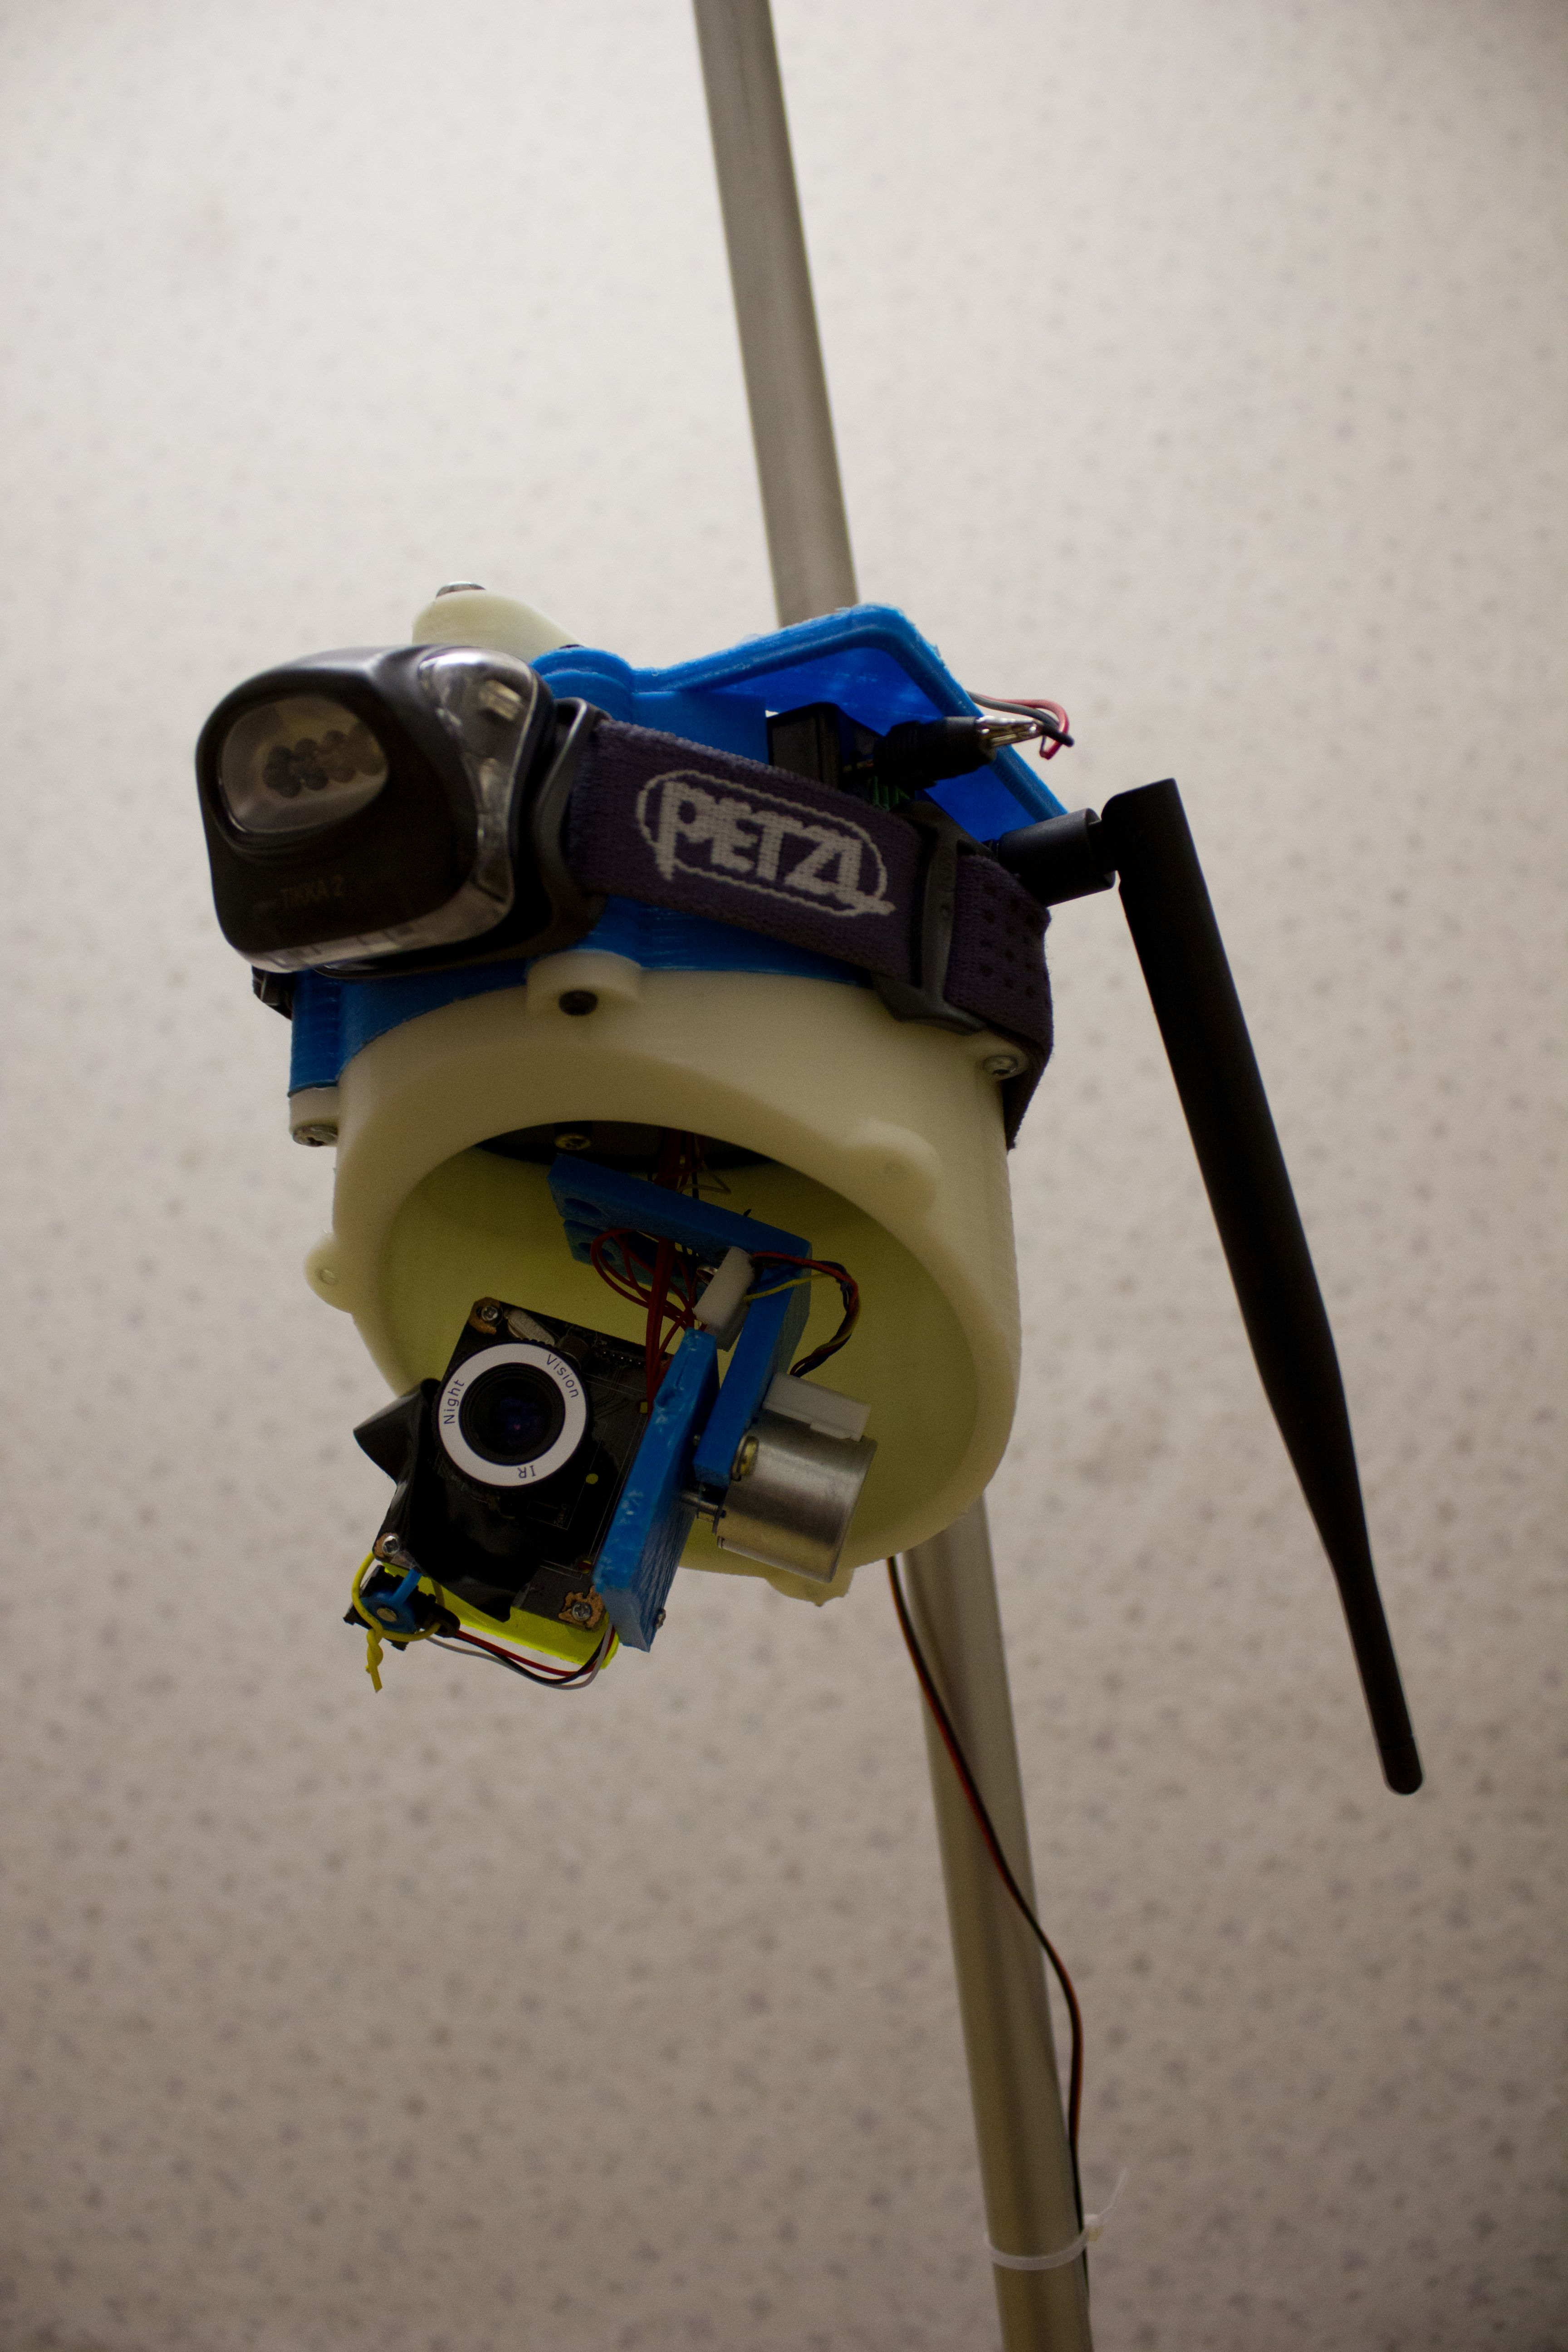
\includegraphics[height=7.5cm]{Besenstiel.jpg}	
}
\frame{\frametitle{Computeraufbau}
	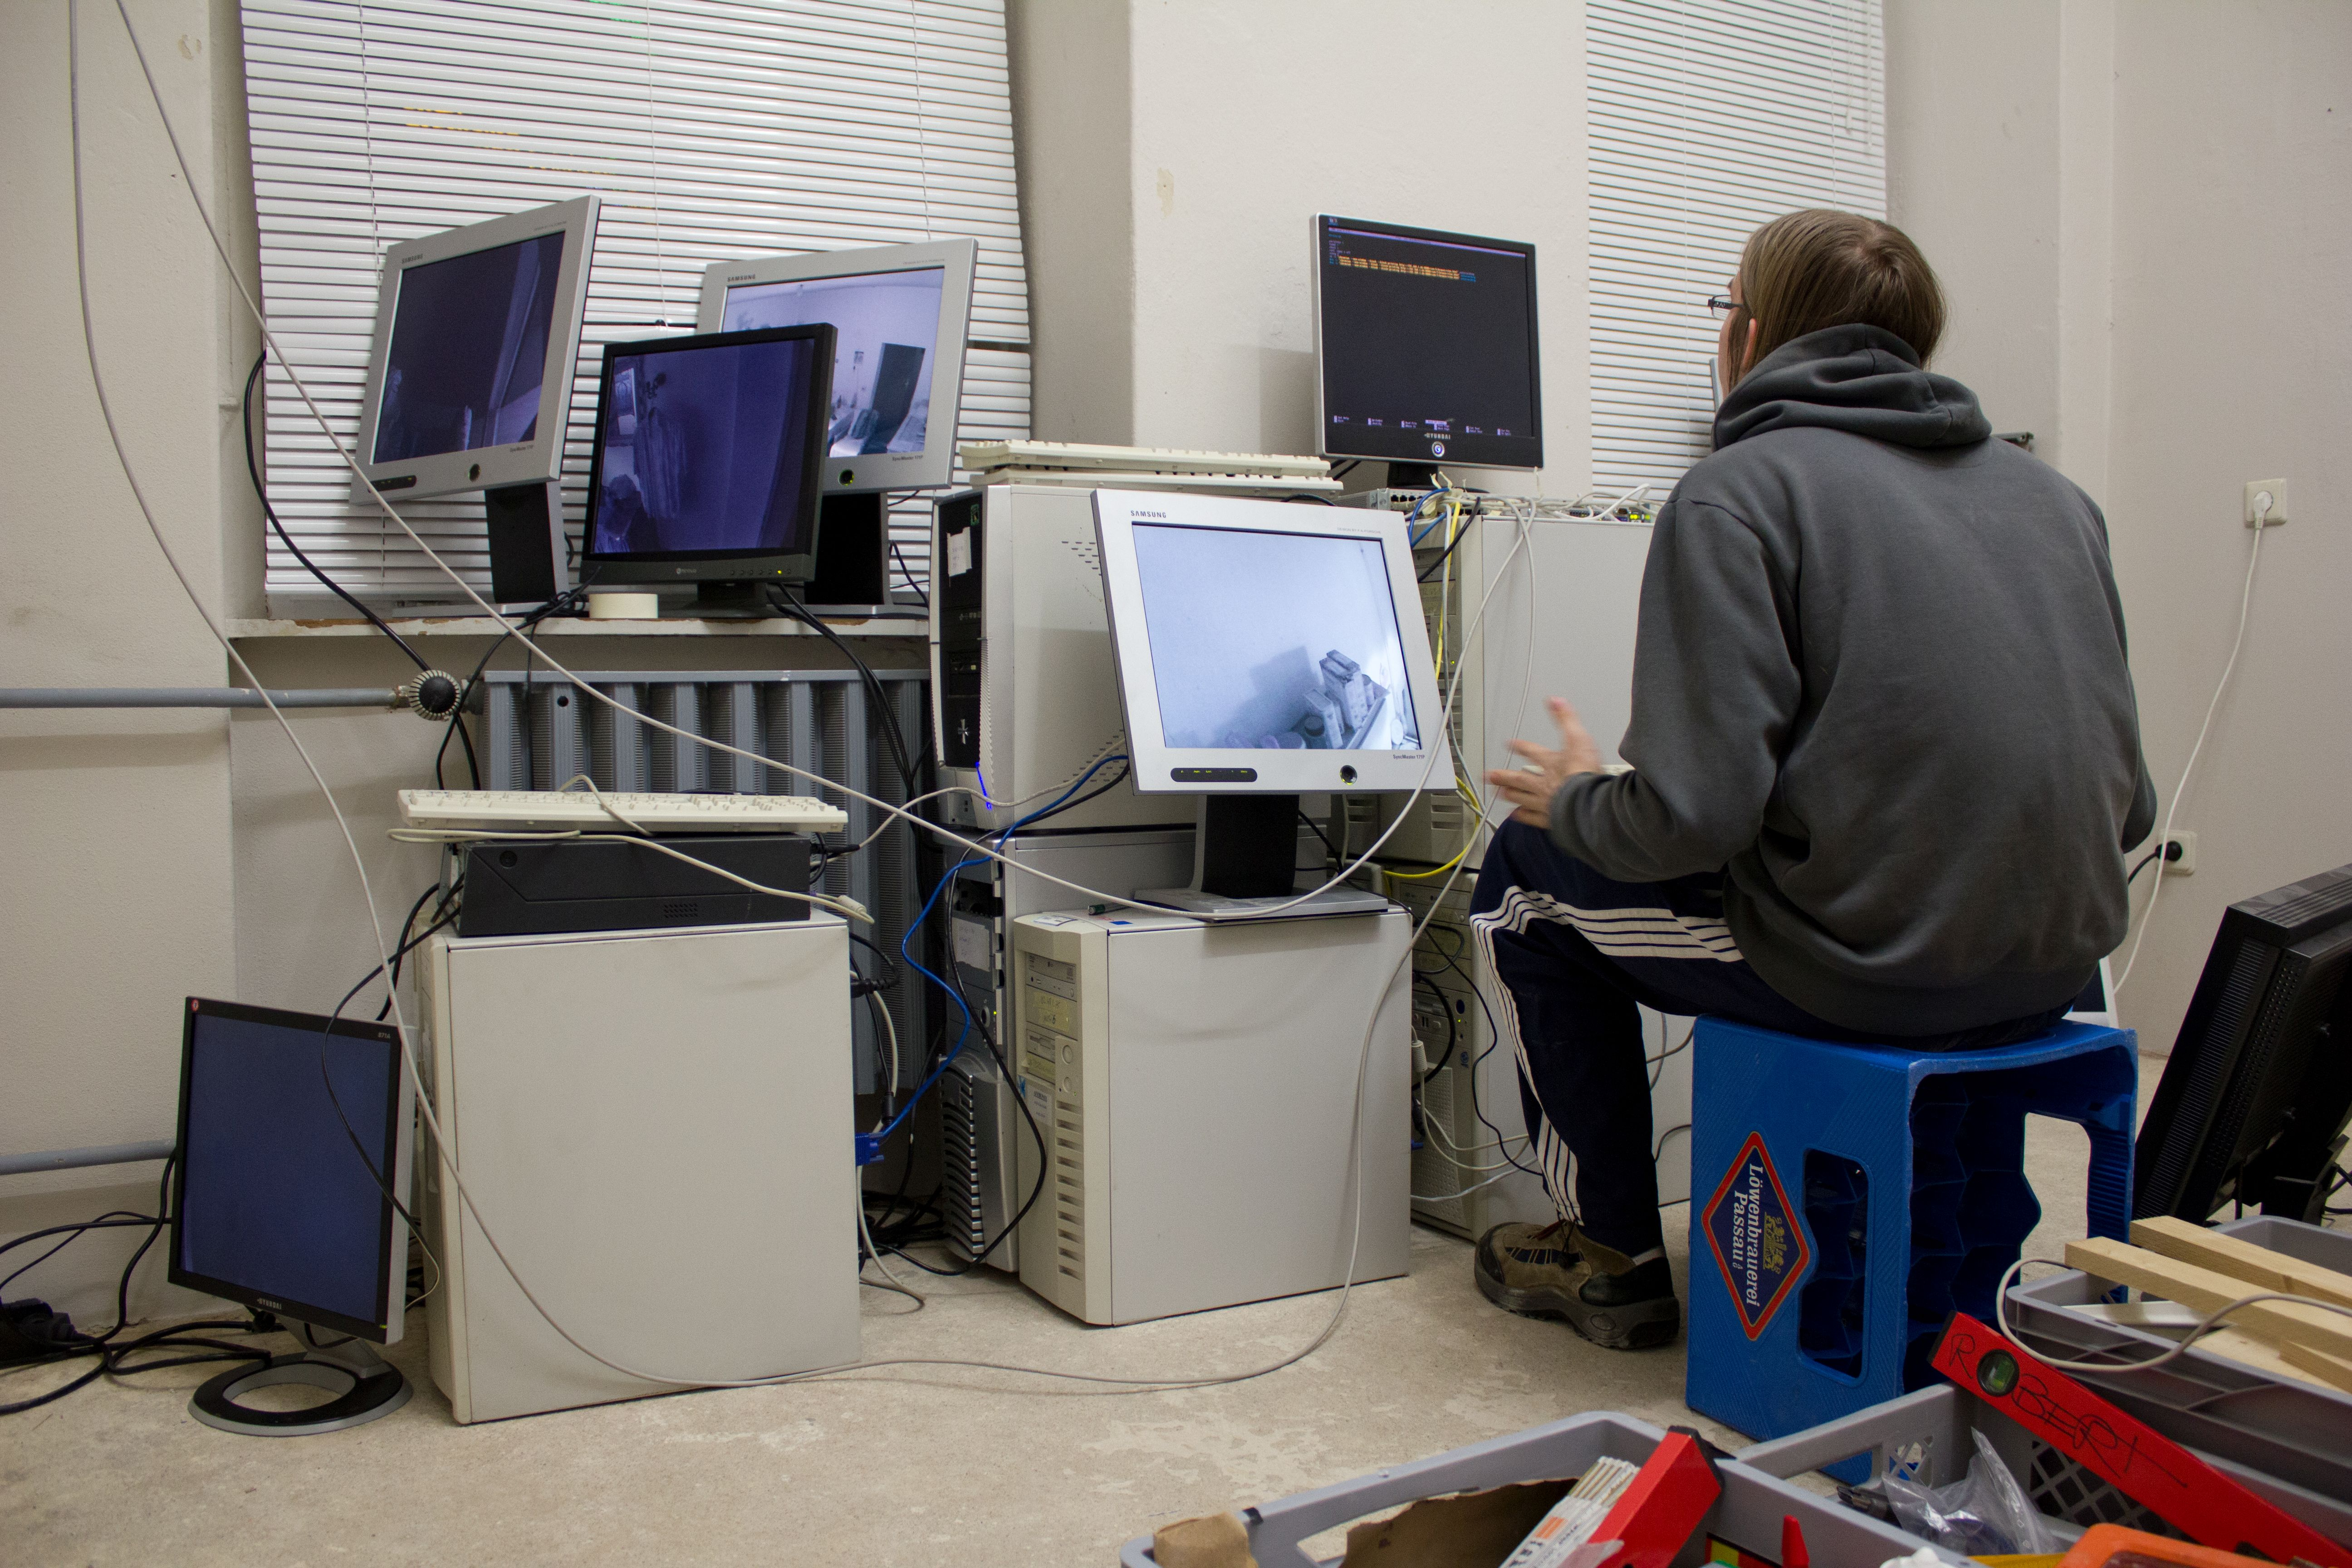
\includegraphics[width=10cm]{ComputerZusammen.jpg}	
}
\frame{\frametitle{�berwachungsstation -- Backstage}
	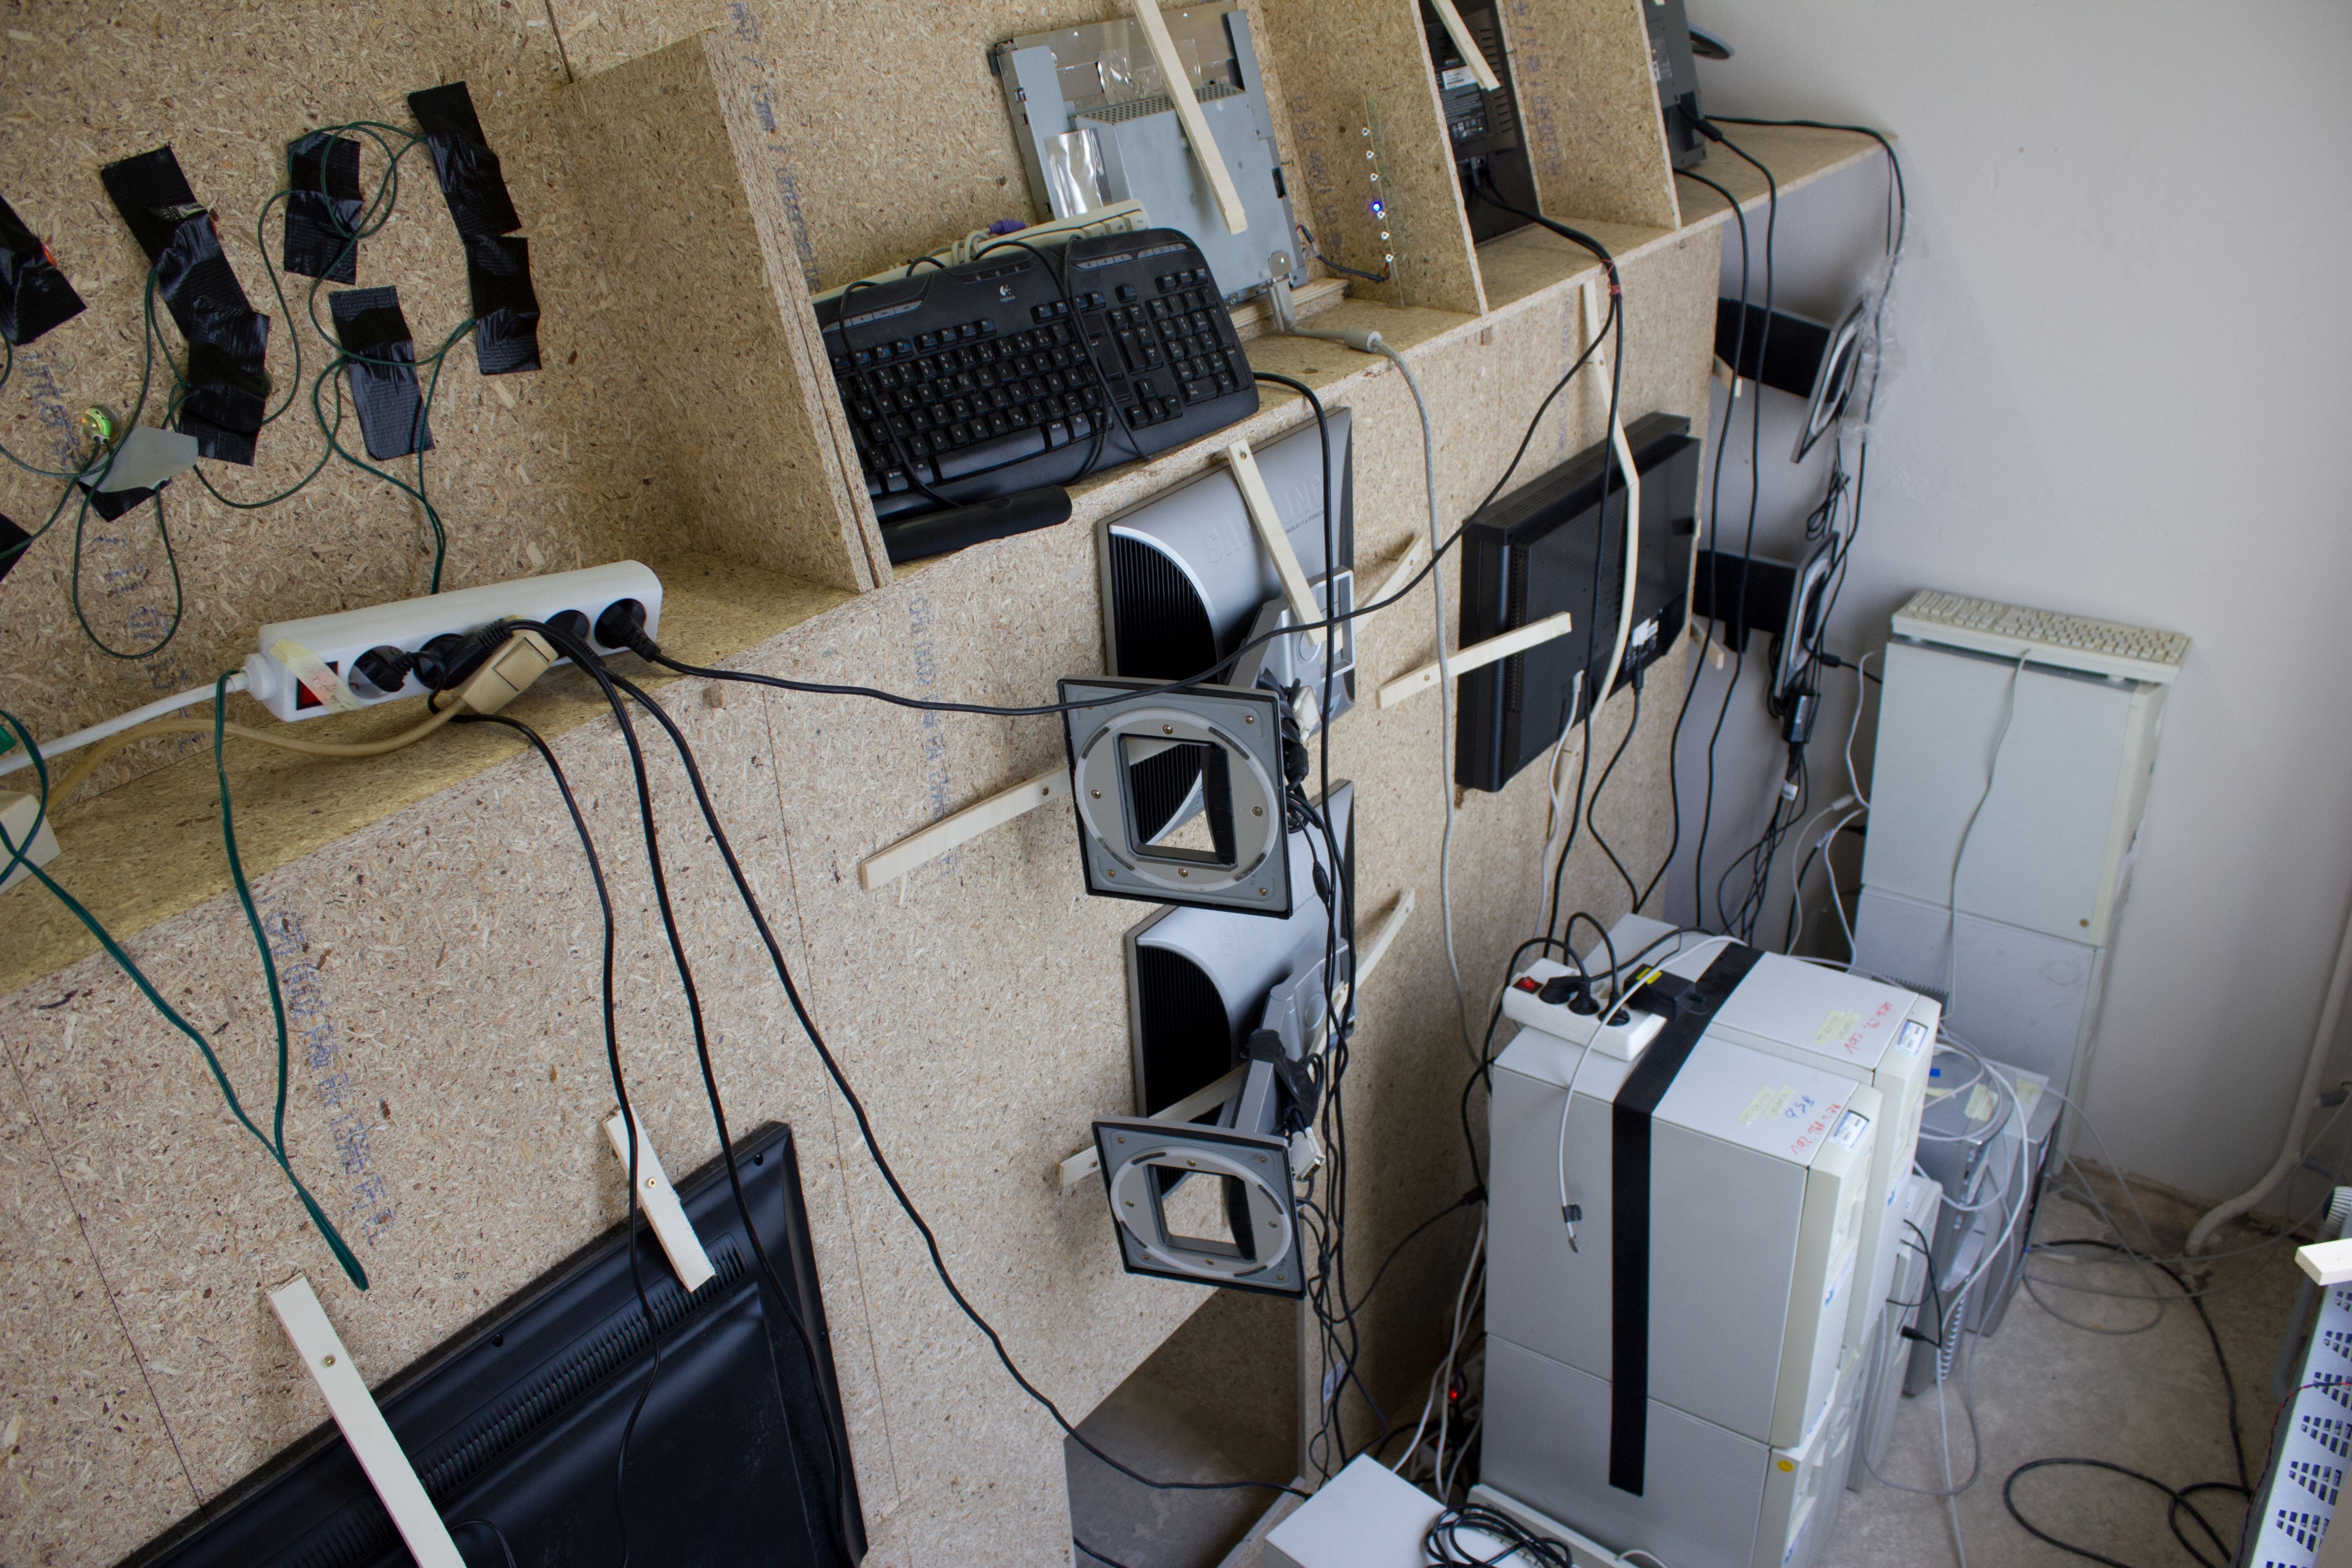
\includegraphics[width=10cm]{Station_h.jpg}	
}

\section{Aufbau}
\frame
{
\frametitle{Aufbau -- Datennetz Roboter }
	\begin{tikzpicture}[->,shorten >=1pt,auto,node distance=4cm,thick,minimum height=1.2cm]
		\node[draw]	(robo)	{Roboter};
		\node[draw] (roboctl) [left of=robo] {Steuerung};
		\node[draw]	(PlexerNW) [above of=robo] {Plexer};
		\node[draw]	(PlexerGa) [above of=roboctl] {Plexer};
		\node[fill=blue!20, minimum height=7cm,minimum width=2cm,label={[label distance=-1cm]90:Funk}] (radio)	at ($(roboctl)!0.5!(PlexerNW)$) {};
		\node[draw] (printer) [left of=PlexerGa,node distance=2cm]	{Drucker};
		\node[draw] (keyboard) [left of=roboctl, node distance=2.5cm,minimum height=0.6cm,minimum width=1.9cm] {Tastatur};
		\node[draw] (joystick) [above of=keyboard, node distance=0.7cm,minimum height=0.6cm,minimum width=1.9cm] {Joystick};
		\node[draw] (monitor) [below of=keyboard, node distance=0.7cm,minimum height=0.6cm,minimum width=1.9cm] {Monitor};
		\node[draw] (nsa)	[right of=PlexerNW, node distance=2cm] {NSA};
		\path[every node/.style={font=\sffamily\small}]
			(roboctl) edge node {Steuerbefehle} (robo)
			(robo)	edge node {Video}	(PlexerNW)
			(PlexerNW) edge node {Video} (PlexerGa)
			(PlexerGa) edge node {Video} (roboctl)
			(PlexerNW) edge node[rotate=45,pos=0.8] {Sperrsignal} (roboctl)
			(PlexerGa) edge (printer)
			(roboctl) edge (monitor)
			(keyboard) edge (roboctl)
			(joystick) edge (roboctl)
			(roboctl) edge [bend left] node {Drucken}	(PlexerGa)
			(PlexerNW) edge [bend left] node {Video} (nsa)
			(nsa) edge [bend left] node {Sperre} (PlexerNW);
			
	\end{tikzpicture}
}
\section{Aufzeichnung}
\frame{\frametitle{Aufzeichnung}
	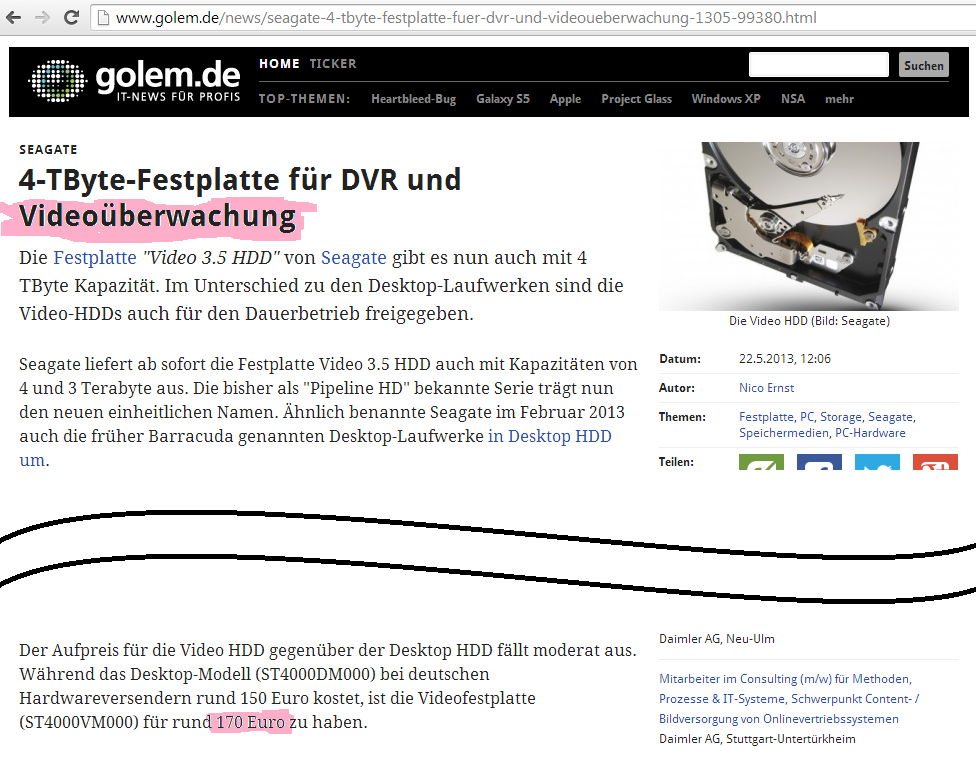
\includegraphics[width=10cm]{HDDueberwachung.png}	
}
\frame{\frametitle{Aufzeichnung}
	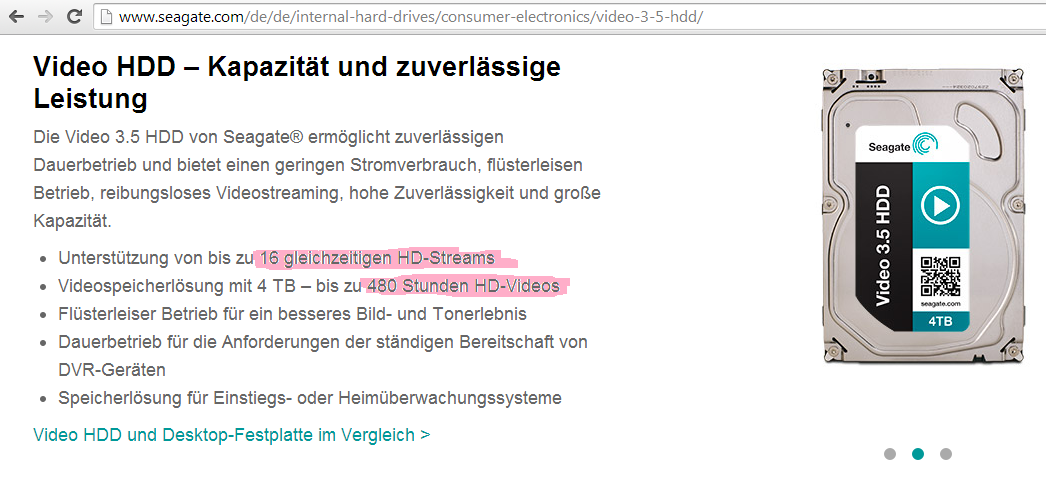
\includegraphics[width=10cm]{HDDueberwachung2.png}	
}
\section{Die �berwachungsstation}
\frame{\frametitle{�berwachungsstation}
	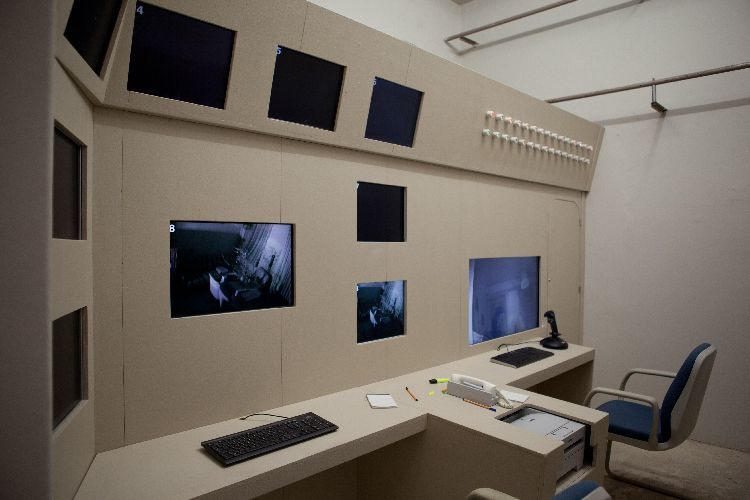
\includegraphics[width=10cm]{Station_v.jpg}	
}





% ----------------------------------------------------------------

\end{document}


\section{Menschen}
\frame
{
\frametitle{Menschen -- Leipzig}
	\textbf{Initiatoren}
	\begin{itemize}
		\item Eva Olivin -- Kaffee, PCs installieren, Flyer, Antr�ge, Abrechnung, Videoschnitt
		\item Robert Verch -- Webseite, PCs installieren, Flyer, Antr�ge, Abrechnung, Videoschnitt
	\end{itemize}
	\textbf{Sublab e.V.}
	\begin{itemize}
		\item Canci -- mjpegplexer (Video)
		\item Olf -- Kamera, Untersuchungsprotokoll
	\end{itemize}
}

\frame
{
\frametitle{Menschen -- Chemnitz}
	\textbf{Chaoschemnitz e.V.}
	\begin{itemize}
		\item Stefan Helmert -- Ladeger�t, Akkus, Robomechanik, -software (Server, Client), Killswitch, Pr�sentation
		\item Thomas Walz -- Akkus, Roboelektronik, Kamera
		\item Mike Stummvoll -- Akkus, Drucken
		\item Florian Schlegel -- Netzwerk, Speicher/Aufzeichnung
		\item Saturntyp -- Kamera-"'Attrappe"' 
	\end{itemize}
	\textbf{Freifunk Chemnitz e.V.}
	\begin{itemize}
		\item Amadeus Alfa -- Funkstrecke, Routing
		\item Steffen F�rster -- Funkstrecke, Routing
	\end{itemize}
	\textbf{sonstige}
	\begin{itemize}
		\item ein Tischler -- Holzkonstruktion der �berwachungsstation
	\end{itemize}
}
